\documentclass[a4paper,fleqn,usenatbib]{mnras}
\usepackage[T1]{fontenc}
\usepackage{ae,aecompl}


\usepackage{graphicx}	% Including figure files
\usepackage{amsmath}	% Advanced maths commands
\usepackage{amssymb}	% Extra maths symbols
\usepackage{subfig}
\usepackage{array}


\usepackage{multirow}
\usepackage{multicol}
\usepackage{blindtext}
\newcolumntype{?}{!{\vrule width 1pt}}
\newcommand{\Mpch}{\,{\rm Mpc}\,\ifmmode h^{-1}\else $h^{-1}$\fi}
\newcommand{\kpch}{\,{\rm kpc}\,\ifmmode h^{-1}\else $h^{-1}$\fi}
\newcommand{\kpc}{\,{\rm kpc}\,}


\newenvironment{Table}
   {\par\bigskip\noindent\minipage{\columnwidth}\centering}
   {\endminipage\par\bigskip}

\title[Dark Matter halo shape in the AURIGA simulations]{The shape of dark matter
  halos in the AURIGA simulations}  
\author[Jesus Prada,  Jaime E. Forero-Romero, Volker Springel ]{
Jesus Prada,$^{1}$\thanks{E-mail: jd.prada1760@uniandes.edu.co}
Jaime E. Forero-Romero,$^{1}$
Volker Springel$^{2}$
\\
% List of institutions
$^{1}$Departamento de F\'sica, Universidad de los Andes, Cra. 1 No.
18A-10, Edificio Ip, Bogot\', Colombia.\\
$^{2}$Heidelberg Institute for Theoretical Studies, Schloss-Wolfsbrunnenweg 35, D-69118 Heidelberg
Germany.\\
}

% These dates will be filled out by the publisher
\date{Accepted XXX. Received YYY; in original form ZZZ}

% Enter the current year, for the copyright statements etc.
\pubyear{2018}

% Don't change these lines
\begin{document}
\label{firstpage}
\pagerange{\pageref{firstpage}--\pageref{lastpage}}
\maketitle

% Abstract of the paper
\begin{abstract}
We measure the shape of the dark matter halos of Milky Way type galaxies.
\end{abstract}

% Select between one and six entries from the list of approved keywords.
% Don't make up new ones.
\begin{keywords}
keyword1 -- keyword2 -- keyword3
\end{keywords}

%%%%%%%%%%%%%%%%%%%%%%%%%%%%%%%%%%%%%%%%%%%%%%%%%%

%%%%%%%%%%%%%%%%% BODY OF PAPER %%%%%%%%%%%%%%%%%%

\section{Introduction}


A robust prediction of the Cold Dark Matter (CDM) paradigm is that DM
halos are ellipsoidal and can be characterized by the principal axes
$a>b>c$.
This ellipsoidal shape is mostly due to the anisotropical and
clumpy accretion of matter influenced by environmental structures.
Numerical studies how that the shape has a strong mass dependence
\citep{Allgood_et_al._2006}, halos are also rounder at the outerskirts
than at the inner part. 
Shape also evolves with cosmic time, halos get
rounder as they evolve.  

There is however a high degree of uncertainty on what is the degree of
uncertainty on the degree of ellipticity of the Milky Way DM halo.
This problem has been addressed both by observations and simulations.
The difficulty in making an observational measurement lies in the
indirect nature of the effect; i.e. the ellipticity can only be
constrained by its effects on quantities such as stellar radial
velocities.
In simulations the uncertainty on predicting the MW DM ellipticity is 
driven by the different physical effects that should be modeled and
its different possible numerical implementations.


Observationally some studies prefer oblate (i.e. a=b>c) configurations at small
distances around $\leq 20$ kpc
\citep[see][]{Law_and_Majewski_2010,Bovy_et_el._2016,Loebman_et_al._2012,Olling_and_Merrifield_2000,Banerjee_and_Chanda_2011} 
and more triaxial and prolate configurations on the outter distances
$\geq 20$ kpc 
\citep[see][]{Vera-Ciro_and_Helmi_2013,Law_and_Majewski_2009,Deg_and_Widrow_2013,Banerjee_and_Chanda_2011}.
However, some  studies are inclined towards prolate configurations even at the inner
parts of the halo \citep[see][]{Bowden_et_al._2016}, and
although it previously seemed that a triaxial DM halo on the
outerskirts would be necessary to fully explain the characterization
of the Sagittarius stream \citep{Law_and_Majewski_2009}, recent studies
questioned this claim by reporting inconsistencies with narrow stellar
streams \citet{Pearson_et_al._2015} or finding that
the relaxation of other constraints may make this claim unnecessary
\citet{Ibata_et_al._2013}. 

In simulations there is strong evidence claiming that the presence of
baryons produces axisymmetrical halos.  
For instance, some studies have shown that the DM halo shape must be
axisymmetrical to ensure the stability of a hydrodynamical disk
embeded in a static DM halo. 
Other have studied this rounding effect by simulating the disk as rigid
potential inside an N-body triaxial DM
halo \cite{Debattista_et_al._2008,Debattista_et_al._2013,Kazantzidis_et_al._2010}
finding that the halo responds to the disk by becoming less triaxial. 

The caveat of the studies mentioned above is that they do not
follow baryons in the whole cosmological context. 
Other studies overcome this limitation by using resimulations 
\citep{Abadi_et_al._2010,Bryan_et_al._2013} finding that the
feeback related to star formation in the disk drives the strenght of
the round effect. 
Recently \cite{2018arXiv180907255C} made a study in a cosmological
simulation to compare the effect of including baryons. They do find,
on average, rounder halo shapes once hydrodynamic effects are
included, but it is uncertain the strenght of this statistical effect
on galaxies similar to the MW.


All these difficulties (enough numerical resolution, explicit
cosmological context, appropriate feedback physics to produce
realistic MW disks) have limited the studies that want to study the
rounding effect of baryons in MW-like galaxies.
In this work we overcome all these limitations by analyzing the
results of state-of-the-art hydrodynamical simulations of isolated
halos that resemble the Milky Way.
We also perform a convergence study with simulation performed at
different resolution levels and explicitly compare the role of DM only
vs. DM+hydro on the MW DM halo shape.

\begin{table*}
\centering
\begin{tabular}{l|cc|cc|cc|cc}
\hline
\hline
Halo & \multicolumn{2}{c}{$N_P$/$10^6$} & \multicolumn{2}{c}{$M_P$/$10^5M_\odot$} & 
\multicolumn{2}{c}{$R_{vir}$/kpc} & \multicolumn{2}{c}{$M_{vir}$/$10^{14} M_\odot$}  \\ \hline
& DM & MHD& DM & MHD& DM & MHD& DM & MHD\\ \hline \hline
halo 1&4.068&2.447&2.397&2.022&196.927&187.674&9.062&7.844\\
halo 2&5.625&5.457&2.481&2.093&235.094&233.934&15.418&15.191\\
halo 3&3.826&3.852&2.645&2.231&210.693&210.955&11.099&11.141\\
halo 4&4.585&4.530&2.590&2.185&219.378&215.438&12.529&11.866\\
halo 5&3.262&3.290&2.533&2.137&196.984&197.246&9.071&9.106\\ 
halo 6 ($\star$)&3.184&3.110&2.337&1.972&191.840&189.342&8.378&8.054\\ 
halo 7&3.878&3.729&2.296&1.937&197.864&196.509&9.193&9.005\\
halo 8&2.772&2.796&2.451&2.068&190.716&191.764&8.231&8.368\\
halo 9&3.038&3.010&2.738&2.310&195.826&190.640&8.911&8.222\\
halo 10&2.700&2.751&2.541&2.144&187.139&188.147&7.777&7.904\\
halo 11&4.146&4.116&2.541&2.144&221.821&219.568&12.952&12.560\\
halo 12&2.865&2.908&2.645&2.231&192.280&192.038&8.436&8.404\\
halo 13&3.520&3.600&2.393&2.019&202.139&203.815&9.801&10.048\\
halo 14&4.200&4.475&2.499&2.108&215.535&218.927&11.882&12.453\\
halo 15&2.888&2.845&2.541&2.144&199.848&200.658&9.471&9.588\\ 
halo 16 ($\star$)&3.821&3.871&2.499&2.108&212.590&212.632&11.401&11.408\\ 
halo 17&2.752&2.781&2.552&2.153&188.067&187.404&7.893&7.811\\
halo 18&3.770&3.624&2.738&2.310&201.124&207.293&9.655&10.571\\
halo 19&2.989&3.086&2.645&2.231&200.244&200.325&9.527&9.540\\
halo 20&3.903&3.822&2.481&2.093&210.097&211.423&11.005&11.214\\ 
halo 21 ($\star$) &4.105&4.075&2.640&2.227&219.527&219.823&12.555&12.604\\ 
halo 22&2.794&2.766&2.625&2.215&188.363&184.801&7.931&7.489\\ 
halo 23 ($\star$) &3.977&4.073&2.795&2.358&217.768&215.959&12.254&11.952\\
halo 24 ($\star$) &4.466&4.426&2.522&2.127&217.440&215.147&12.199&11.817\\ 
halo 25&2.902&2.806&2.645&2.231&199.922&198.299&9.482&9.254\\
halo 26 &4.610&4.716&2.506&2.115&219.984&218.939&12.633&12.454\\
halo 27 ($\star$) & 5.060&5.018&2.590&2.185&228.036&226.225&14.071&13.740\\ 
halo 28 & 4.184&4.276&2.645&2.231&216.979&217.997&12.121&12.294\\
halo 29 & 4.827&4.613&2.499&2.108&225.791&219.935&13.660&12.625\\
halo 30 & 3.268&3.112&2.579&2.176&195.043&194.741&8.805&8.763\\
\hline
\hline
\end{tabular}
\caption{Specifications of each level 4 galaxy (halo). 
  The DM and MHD versions of each parameters are presented together. 
  The columns correspond to: (1) Halo name, (2,3) Millions of DM
  particles belonging to the halo, (4,5) DM particle mass in
  $10^5M_\odot$, (6,7) Halo Virial radius in kpc and (8,9) halo virial
  mass in $10^{14}M_\odot$. Halos marked with a star ($\star$) are
  correspond to halos resimulated at higher resolution (level 3).}  
\label{tab:level4}
\end{table*} 

\begin{table*}
\centering
\begin{tabular}{l?cc?cc?cc?cc}
\hline
\hline
Halo & \multicolumn{2}{c?}{$N_P$/$10^6$} & \multicolumn{2}{c?}{$M_P$/$10^5M_\odot$} & \multicolumn{2}{c?}{$R_{vir}$/kpc}&\multicolumn{2}{c}{$M_{vir}$/$10^{14}M_\odot$}  \\ \hline
& DM & MHD& DM & MHD& DM & MHD& DM & MHD\\ \hline \hline
halo 6&24.902&24.185&0.292&0.246&191.741&188.367&8.365&7.932\\
halo 16&29.750&30.334&0.312&0.263&212.622&212.542&11.406&11.395\\
halo 21&31.993&31.503&0.330&0.278&219.731&220.250&12.588&12.679\\
halo 23&31.379&31.618&0.349&0.295&217.793&213.358&12.259&11.524\\
halo 24&34.987&35.153&0.315&0.266&217.313&213.963&12.179&11.624\\
halo 27&39.617&39.056&0.324&0.273&227.908&223.484&14.048&13.244\\
\hline
\hline
\end{tabular}
\caption{Same layout Table \ref{tab:level3} for Level 3 simulations (higher
  resolution than Level 4 simulations).}
\label{tab:level3}
\end{table*} 



\section{Numerical Simulations}

In this work we use the results of the state-of-the art Auriga
simulations \citep{auriga}. 
The objects in those simulations were selected from a set of 30
isolated halos in the Evolution and Assembly of GaLaxies and their
Environments (EAGLE)  project \citep{Eagle}.   
These halos were randomly selected from a sample of the most isolated
halos whose virial mass $M_{200}$ varied between $10^{12}M_\odot$ and
$2\times 10^{12}M_\odot$. 
These halos were re-simulated with higher resolution an varying
physical realism using the AREPO code \citep{arepo}.
 
All 30 halos were simulated within resolution defined for Aquarius
simulations corresponding to $\sim 3\times 10^6$ high resolution DM
particles of $\sim 2.5 \times 10^5 M_\odot$.  
This resolution is labeled as Level 4, the main details for each halo
are consigned in Table \ref{tab:level4}. 
From these 30 halos, 6 of them where re-simulated at higher resolution
(labeled as Level 3) taking into account a spatial factor of 2 in each
dimension.   
Details of Level 3 halos are in Table \ref{tab:level3}. 
Furthermore, for each halo in each level of resolution there are two
versions of the simulation: DM-only and DM plus baryons with
magneto-hydrodynamical (MHD) physics.  





\begin{figure*}
  \centering
  \subfloat[halo 16 DM shape at small
    radius]{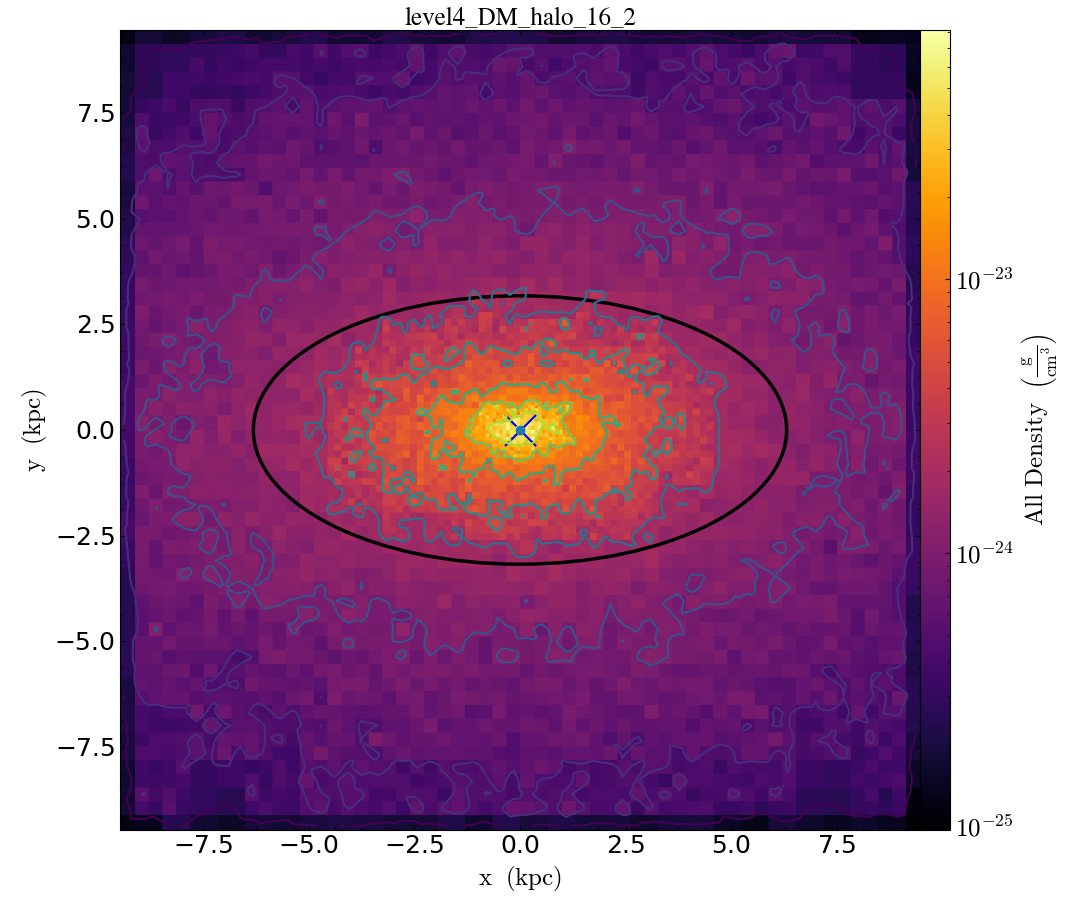
\includegraphics[width=0.5\textwidth]{./pics/MHD_Vs_DM/level4_DM_halo_16_inner.png}} 
  \hfill
  \subfloat[halo 16 DM shape at big
    radius]{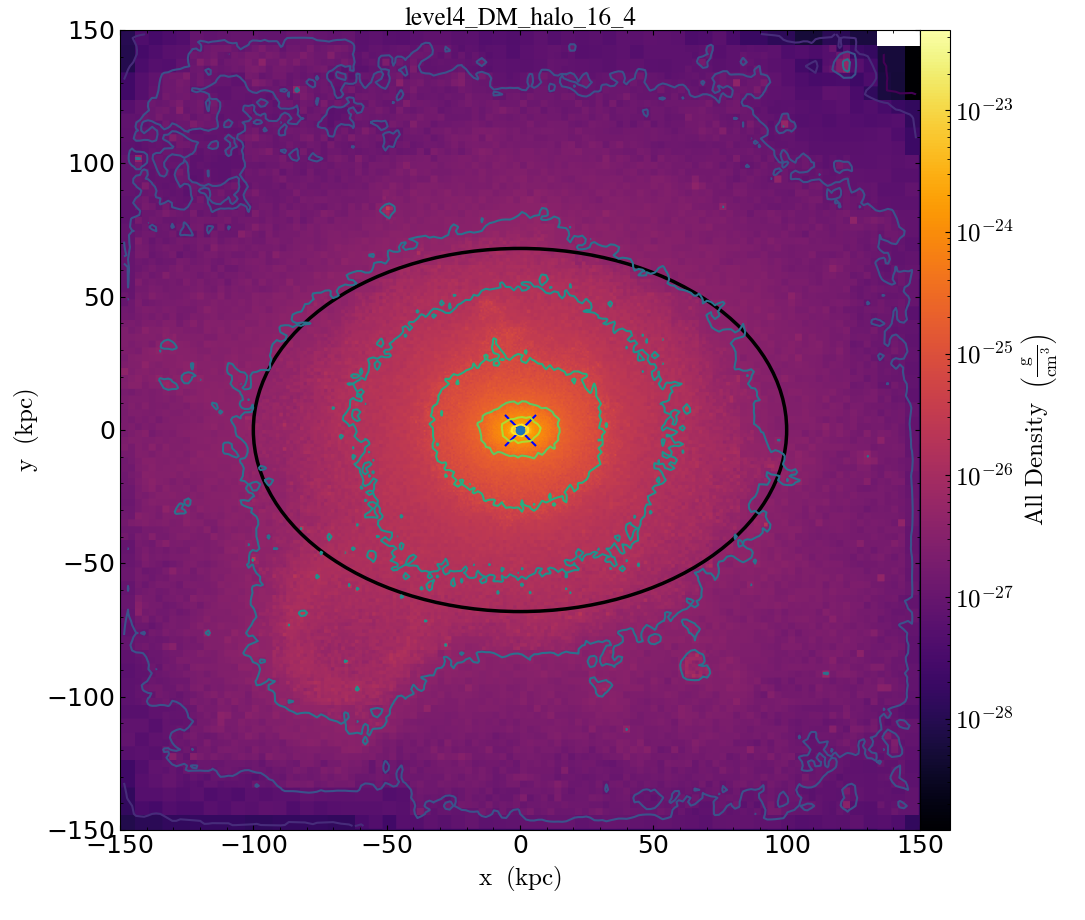
\includegraphics[width=0.5\textwidth]{./pics/MHD_Vs_DM/level4_DM_halo_16_outer.png}} 
  \hfill 
  \caption{DM density for inner/outer (left/right panel) DM halo regions.  
  Slice 20 percent of the max-min range in the "z" position of
  particles belonging to the main structure, centered at halo defined
  position (calculated with most bounded particle) }  
  \label{fig:slices}
\end{figure*}

\section{Determining the halo shape}

%\subsection{The solid ellipsoid method}

The DM halo shape at a fixed radius is an estimate of either
the isopotential or isodensity surfaces.  
Observational inference models usually estimate the 
isopotential contours which are probed by tracers (gas, stars), while
simulations work with the isodensity contours which can be directly
calculated from particle positions.  

However, in numerical simulations the density contours are not smooth
and are sensitive to the presence of small satelites. 
For this reason we choose to measure the shape by taking
volume-enclosed particles, rather than shell-enclosed.  
We follow the shape measurement method presented by
\cite{Allgood_et_al._2006} that uses the reduced
inertia tensor,     

\begin{equation}
I_{ij} = \sum_k \frac{x_k^{(i)}x_k^{(j)}}{d^2_k},
\label{eq:inertia}
\end{equation}

with the positions components weighted by the k-th particle distance
$d_k^2=x_k^2+y_k^2+z_k^2$, the particle positions are measured from
the minimum of the gravitational potential in each halo.
The diagonalization of this tensor yields the principal axes of the
structure as well as the eigen-quantities which are proportional to
the squared principal axes $a>b>c$. 

We start the calculations taking into account particles within a
sphere of radius $R$ and then  recharacterize the triaxial parameters
by taking into account particles within an ellipsoid of semi-axes
$r,r/q,r/s$ and re-scaled distance $d^2=x^2+(y/q)^2+(z/s)^2$, where $q
= b/a$ and $s=c/a$ are the previously calculated axial ratios. 
We repeat this process until the average deviation of semi-axes is
less than $10^{-6}$.  
This is the same method used to estimate the halo shape in the DM-only
Aquarius simulations \citep{Vera-Ciro_et_al._2011}. 

We restrict the sampling of the ellipsoidal parameters to radii
between $1/16 R_{vir}$ and $2R_{vir}$, where  $R_{vir}$ is taken as the
radius enclosing a sphere with 500 times the average dark matter
density of the Universe. 
All our results use of this reference radius
unless strictly stated otherwise. 
We peform the shape measurements both as a function of radius and
redshift for all halos in the sample.


\section{Results}

\subsection{Radial trends at $z=0$}


We find that in DM-only simulations halos are monotonically rounder
with increasing radius, confirming results already reported in the
literature \citep{Vera-Ciro_et_al._2011}. 
Figure \ref{fig:slices} illustrates this effect.
There we show the density a DM-only halo at redshift zero in a thin
slice passing through the halo's centre, each panel shows the halo at
different radii.
The ellipse plotted over the contours indicates the outermost
boundary of the estimated shape ellipsoid. 
Indeed, the ellipse panel on the right (outer halo) is rounder than
the ellipse on the left (inner halo). 


\begin{figure*}
\centering
{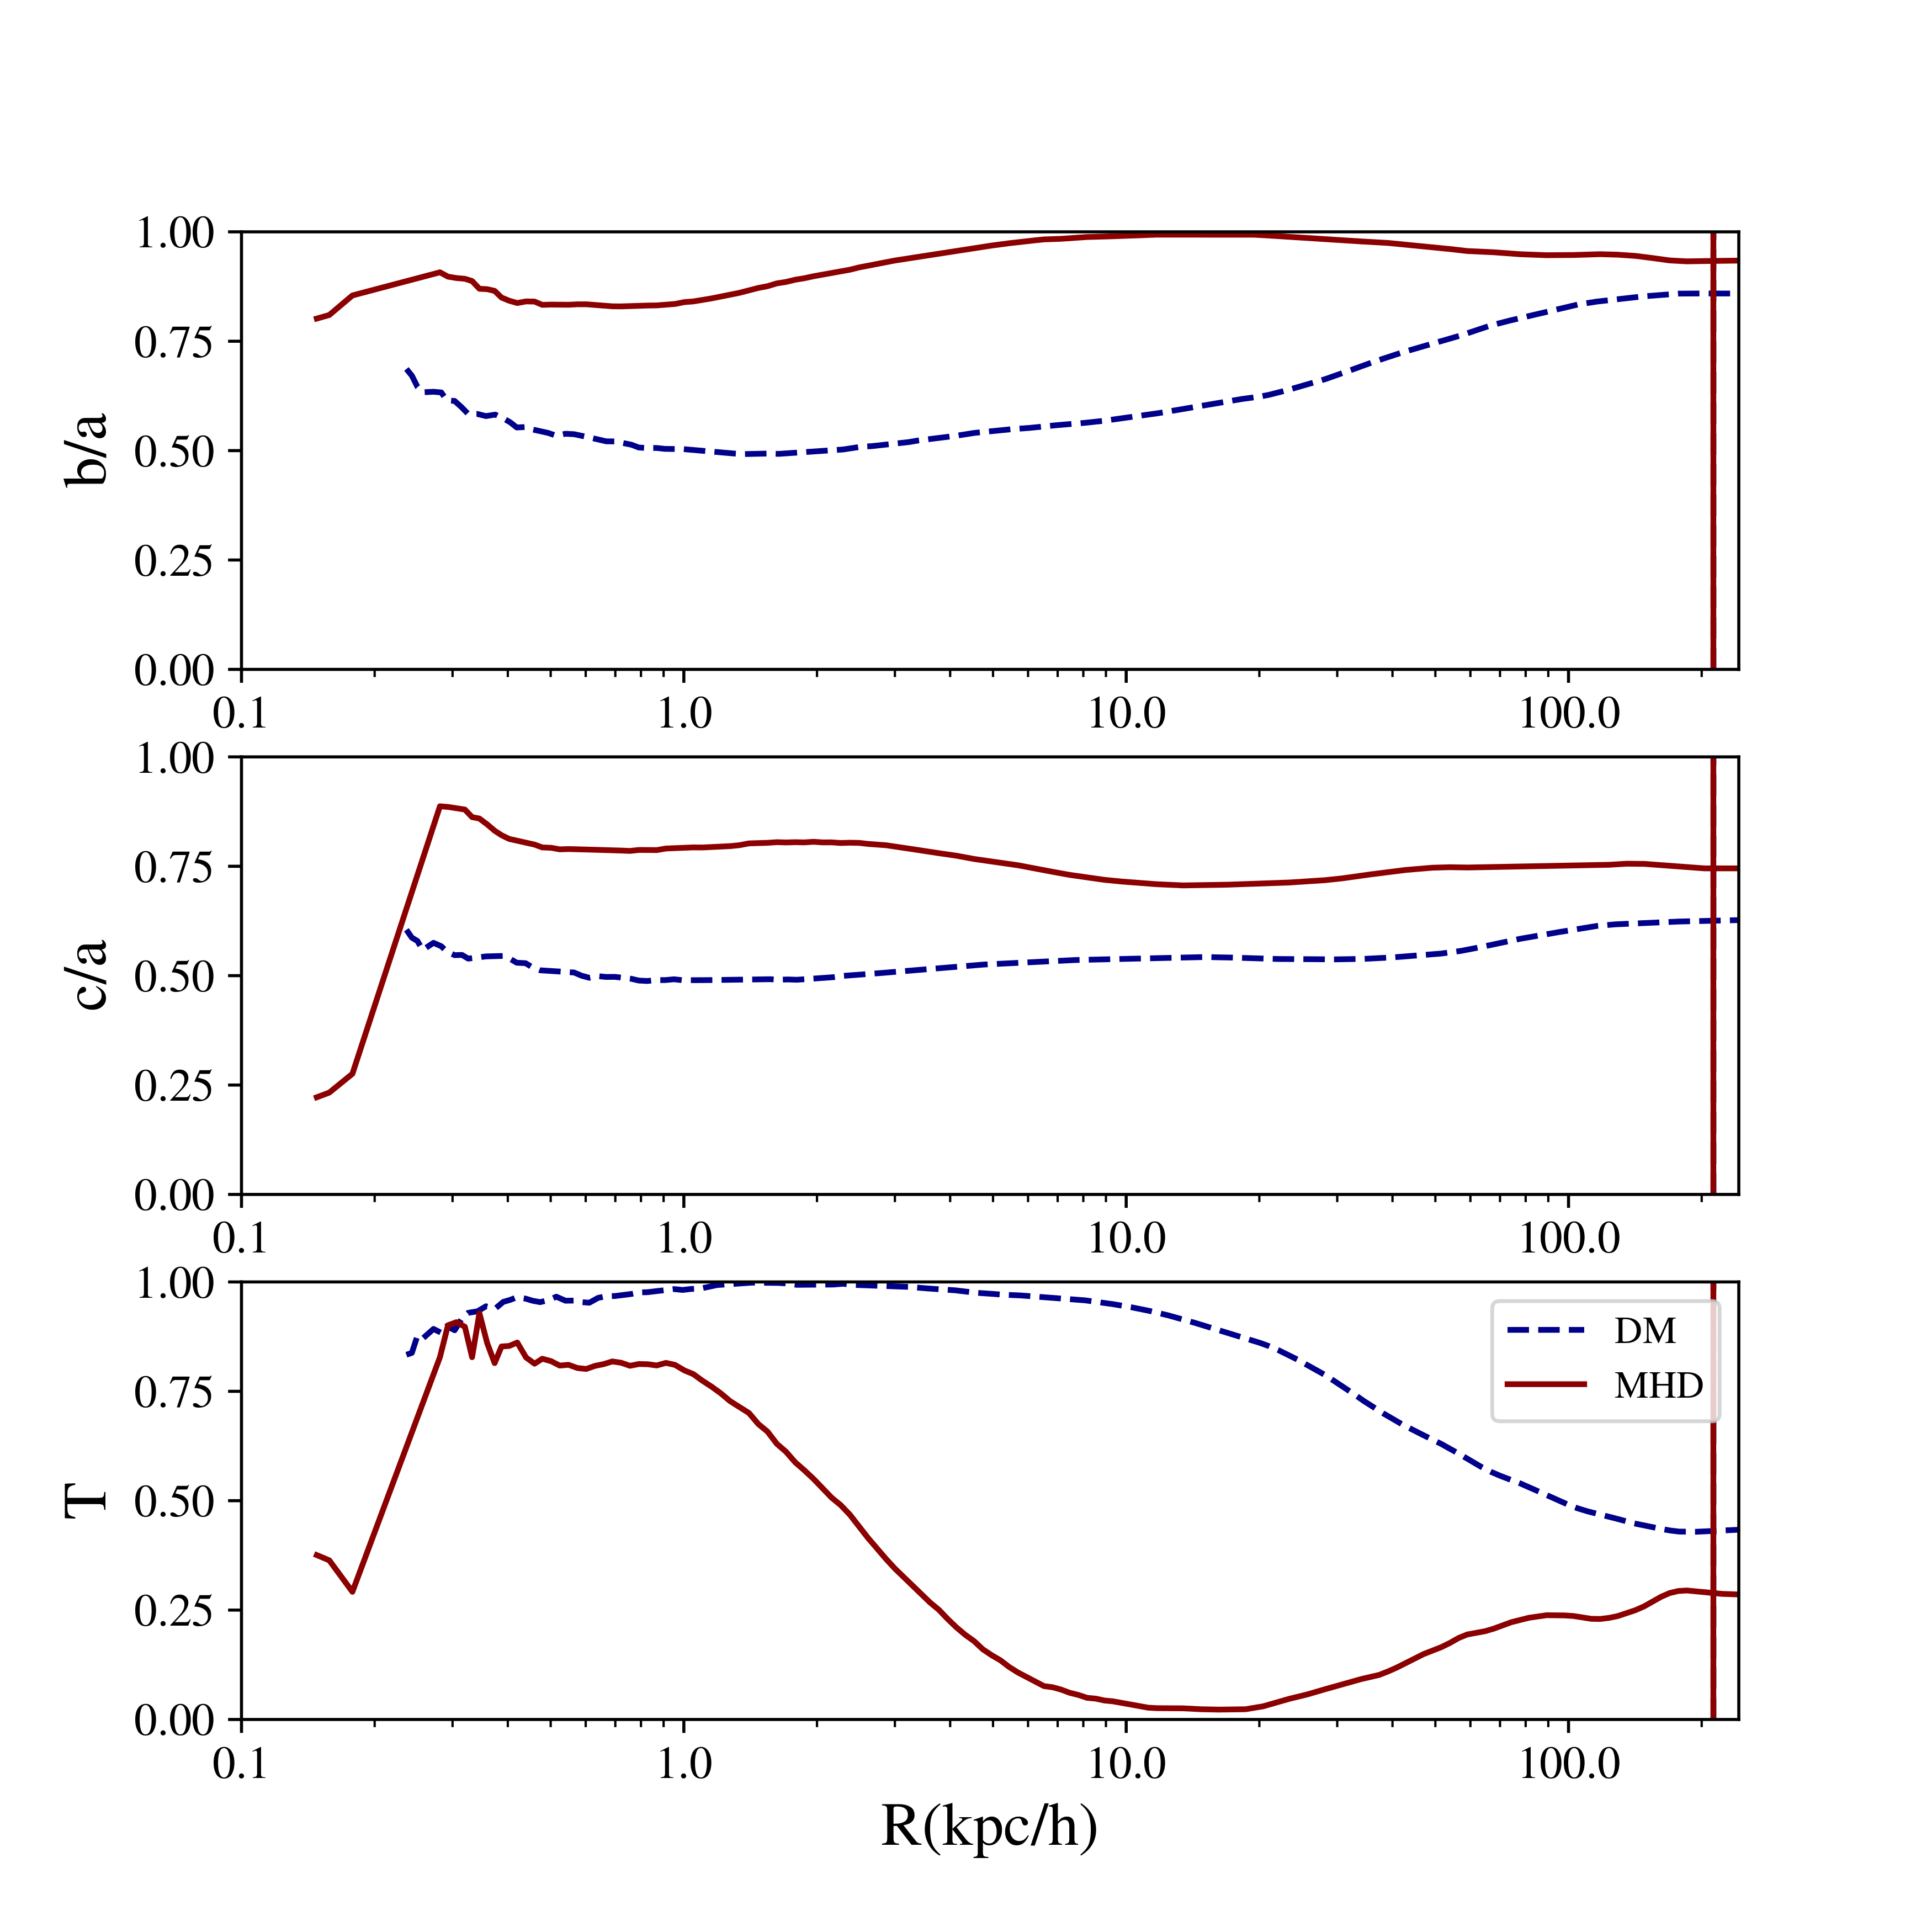
\includegraphics[width=0.6\textwidth]{./pics/MHD_Vs_DM/halo16_new.png}}
\caption{Radial profile for the axial ratios and the triaxiality parameter
  $T=\frac{1-b/a}{1-c/a}$ at redshift $z=0$. 
  Radial profile was sampled at
  redshift 0 and there are two sets of lines showing MHD and DM-only
  versions of the axial ratios profile. {\bf Aqui hay que quiar c/b,
    no es relevante}} \label{fig:triaxial_radius}
\end{figure*} 


We quantify this effect by plotting the axial ratios $q$, $s$,
$s/q$ and the triaxiality $T\equiv \frac{1-q}{1-s}$ as a
function of radius. 
As a representative sample of this relations we show on Figure
\ref{fig:triaxial_radius} the radial trends for Halo 16 at
the highest resolution both for DM and MHD simulations.
The continous lines correspond to the DM simulation and shows how
the inner part of the halo $r\approx 1$\kpch has values of 
$q=0.5$, $s=0.5$ while at the virial radius the same
quantities increase to $q=0.85$, $s=0.6$; in turn the triaxiality
decreases from $T\approx 1.0$ to $T\approx0.4$. 

In the same Figure \ref{fig:triaxial_radius} we also find one of the
main results of our study: halos in MHD simulations are systematically rounder, at
every radius, than its DM-only counterparts.  
The dashed line in Figure \ref{fig:triaxial_radius} shows that at
$r\approx 1$\kpch  in the MHD simulation we have $q=0.85, s=0.8$
($q=0.5, s=0.5$ in DM) and at the virial radius $q=0.95, s=0.75$
($q=0.85, s=0.6$ in DM).  
However, the triaxiality trend is not as monotonous for MHD halos is
it is in DM halos. 
The triaxiality goes almost to zero at an intermediate radius,
$r\approx 10$\kpc in the case of Halo 16 in Figure
\ref{fig:triaxial_radius}, to increase again. {\bf pasa lo mismo para
  todos los halos? es lo mismo para baja y alta resolucion de MHD?}
    

Figure \ref{fig:triax_DM_MHD} summarizes this comparizon for all 30 halos
in the Level 3 simulations. 
Measurements at $R_{\rm vir}/16$ are represented by circles while squares 
are measurements at $R_{\rm vir}$. 
All halos, except two, show that outer regions rounder than inner
regions.
The exceptions are cases where a merging substructures near  the
halo's center gives rise to perturbed axial ratio measurements. 
The right panel on Figure \ref{fig:triax_DM_MHD} shows the same information, this time for
the MHD simulations. 
In this case, the main radial trend continues to hold, albeit less
pronounced.
We also find that halos in MHD simulations are in general rounder than
their DM counterparts


This global behaviour can be also illustrated by the individual case
of Halo 16, shown in Figure \ref{fig:triaxial_radius}.
At the virial radius the halo is rounder than its DM counterpart as
evidenced in the axis ratios $b/a$, $c/a$ and the triaxiality.
In the MHD simulation, going from the virial radius to $10$ \kpch the
$b/a$ ratio is constant almost close to unity while in the DM-only
simulation it decreases to $0.5$.
Between $2$-$10$ \kpc the triaxiality in the DM-only simulation is in
the range $0.9-1.0$, while the MHD simulation has values between
$0-0.5$. 


In Table \ref{table:median_axial_ratio_DM} and Table \ref{table:median_axial_ratio_MHD}
we summarize these trends for the median values of the axis ratio in
the DM and MHD simulations
The lower/upper bounds correspond to the first/third quartiles. 
Table  \ref{table:median_axial_ratio_DM} shows how halos are
monotonically rounder with increasing radius; while the comparison
against Table \ref{table:median_axial_ratio_MHD} shows how DM halos
are consistently rounder in MHD simulations than DM-only runs at every
radius. 


 
\begin{figure*}
\begin{center}
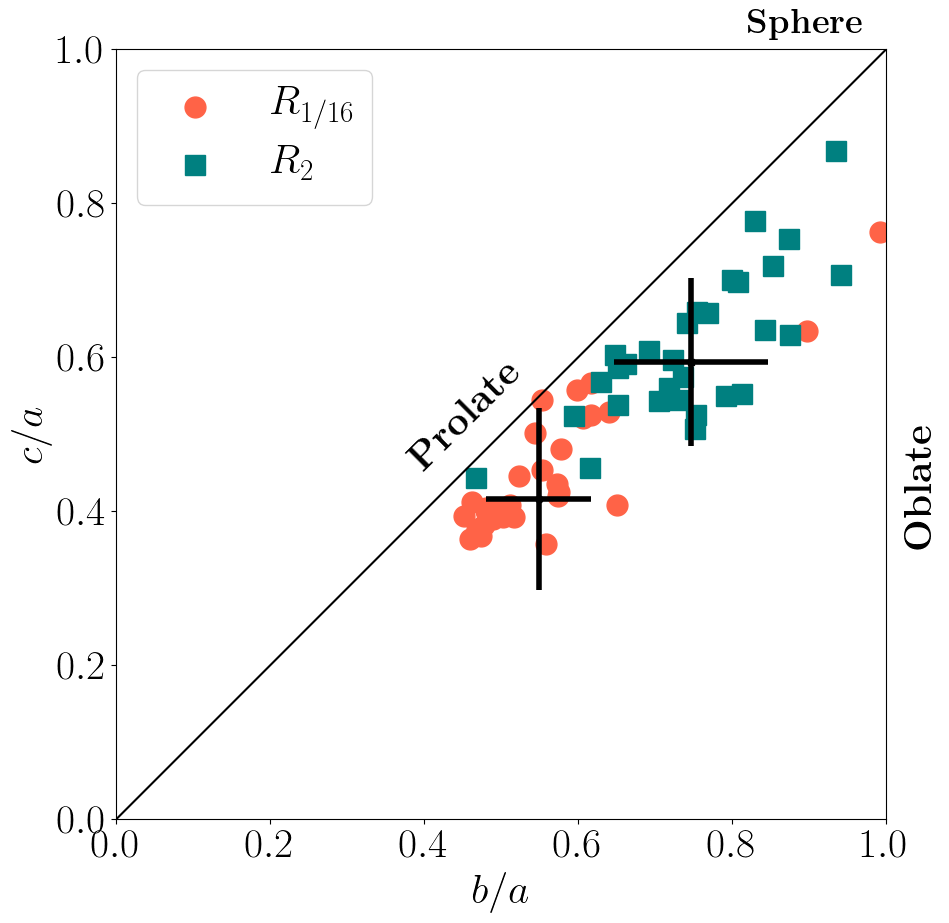
\includegraphics[width=0.9\columnwidth]{./pics/Triaxial_Plane/Triax_DM.png}
 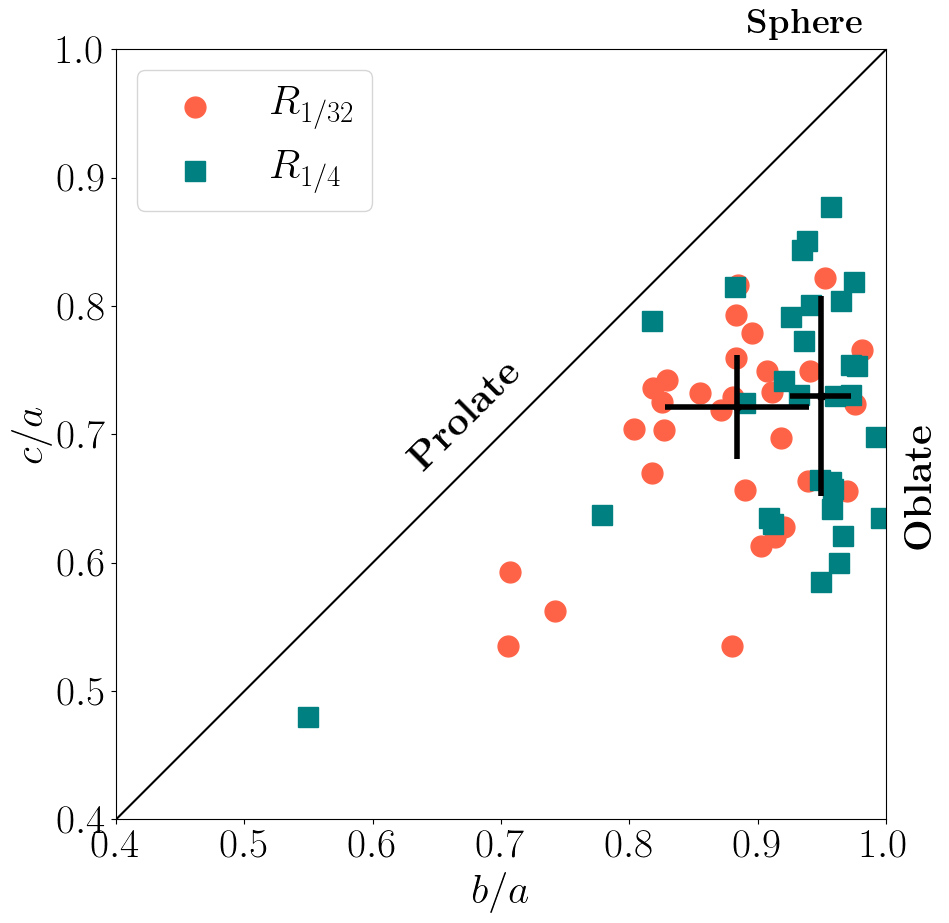
\includegraphics[width=0.9\columnwidth]{./pics/Triaxial_Plane/Triax_MHD.png}
\end{center}
\caption{Axial ratios for the 30 halos in the Level 3 DM simulations
  on the left and MHD simulations on the right.
   Each dot represents the shape characterization of each halo at the
   2 times the virial radius and a  1/16 fraction of the virial radius
   differentiated by color. 
   Errorbar shows median and errors for each sampled radii. 
   Conclusion: DM halos are rounder on the outskirts {\bf Esto necesita
  correccion. Debe ser a R1/16 y R (no 2R!)}}
  \label{fig:triax_DM_MHD}
\end{figure*}



\begin{table}
\setlength{\tabcolsep}{3pt}
\begin{center}
\begin{tabular}{l|ccccc}
 &$R_{1/16}$& $R_{1/8}$& $R_{1/4}$& $R_{1/2}$& $R_1$\\
\hline 
$b/a$ &$0.55^{+0.07}_{-0.07}$&$0.57^{+0.09}_{-0.08}$&$0.61^{+0.15}_{-0.08}$&$0.65^{+0.18}_{-0.10}$&$0.70^{+0.13}_{-0.10}$ \\ [0.1cm]
$c/a$ &$0.42^{+0.12}_{-0.03}$&$0.45^{+0.11}_{-0.04}$&$0.49^{+0.09}_{-0.05}$&$0.52^{+0.10}_{-0.05}$&$0.56^{+0.10}_{-0.05}$\\ [0.1cm]
$T$ &$0.89^{+0.03}_{-0.08}$&$0.88^{+0.04}_{-0.12}$&$0.84^{+0.08}_{-0.23}$&$0.81^{+0.08}_{-0.29}$&$0.75^{+0.14}_{-0.25}$\\ [0.1cm]
\end{tabular}
\end{center}
\caption{Median values of axial ratios $q,s$ and triaxiality parameter
  $T$ for DM halos in DM-only simulations at different radii. The
  median is computed over the 30 halos in Level 3 simulations.}  
\label{table:median_axial_ratio_DM}
\end{table}



\begin{table}
\setlength{\tabcolsep}{3pt}
\begin{center}
\begin{tabular}{l|ccccc}
 &$R_{1/16}$& $R_{1/8}$& $R_{1/4}$& $R_{1/2}$& $R_1$\\
\hline 
$b/a$ &$0.93^{+0.04}_{-0.04}$&$0.95^{+0.03}_{-0.03}$&$0.95^{+0.02}_{-0.05}$&$0.93^{+0.04}_{-0.06}$&$0.93^{+0.04}_{-0.10}$\\[0.1cm]
$c/a$ &$0.73^{+0.05}_{-0.09}$&$0.73^{+0.07}_{-0.10}$&$0.73^{+0.08}_{-0.10}$&$0.73^{+0.09}_{-0.08}$&$0.75^{+0.07}_{-0.11}$\\[0.1cm] 
$T$ &$0.31^{+0.15}_{-0.22}$&$0.20^{+0.24}_{-0.12}$&$0.24^{+0.20}_{-0.12}$&$0.30^{+0.26}_{-0.16}$&$0.36^{+0.23}_{-0.23}$\\[0.1cm] 
\end{tabular}
\end{center}
\caption{Median values of axial ratios $q,s$ and triaxiality parameter
  $T$ for DM halos in MHD-only simulations at different radii. The
  median is computed over the 30 halos in Level 3 simulations.}  
\label{table:median_axial_ratio_MHD}
\end{table}



\subsection{Shape evolution with cosmic time}


\begin{figure*}
  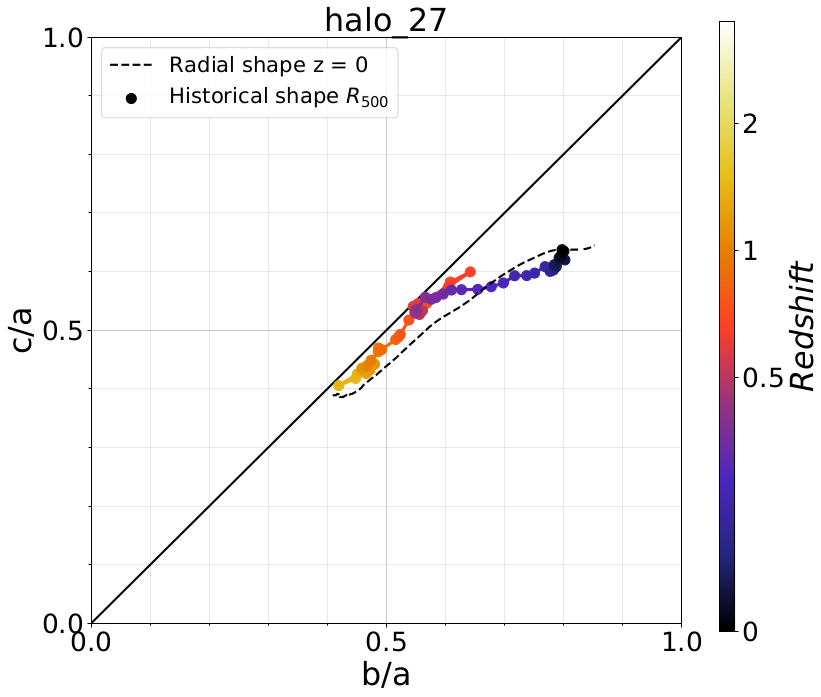
\includegraphics[width=\columnwidth]{./pics/Redshift/halo_27_DM_Z_correlation.png}
  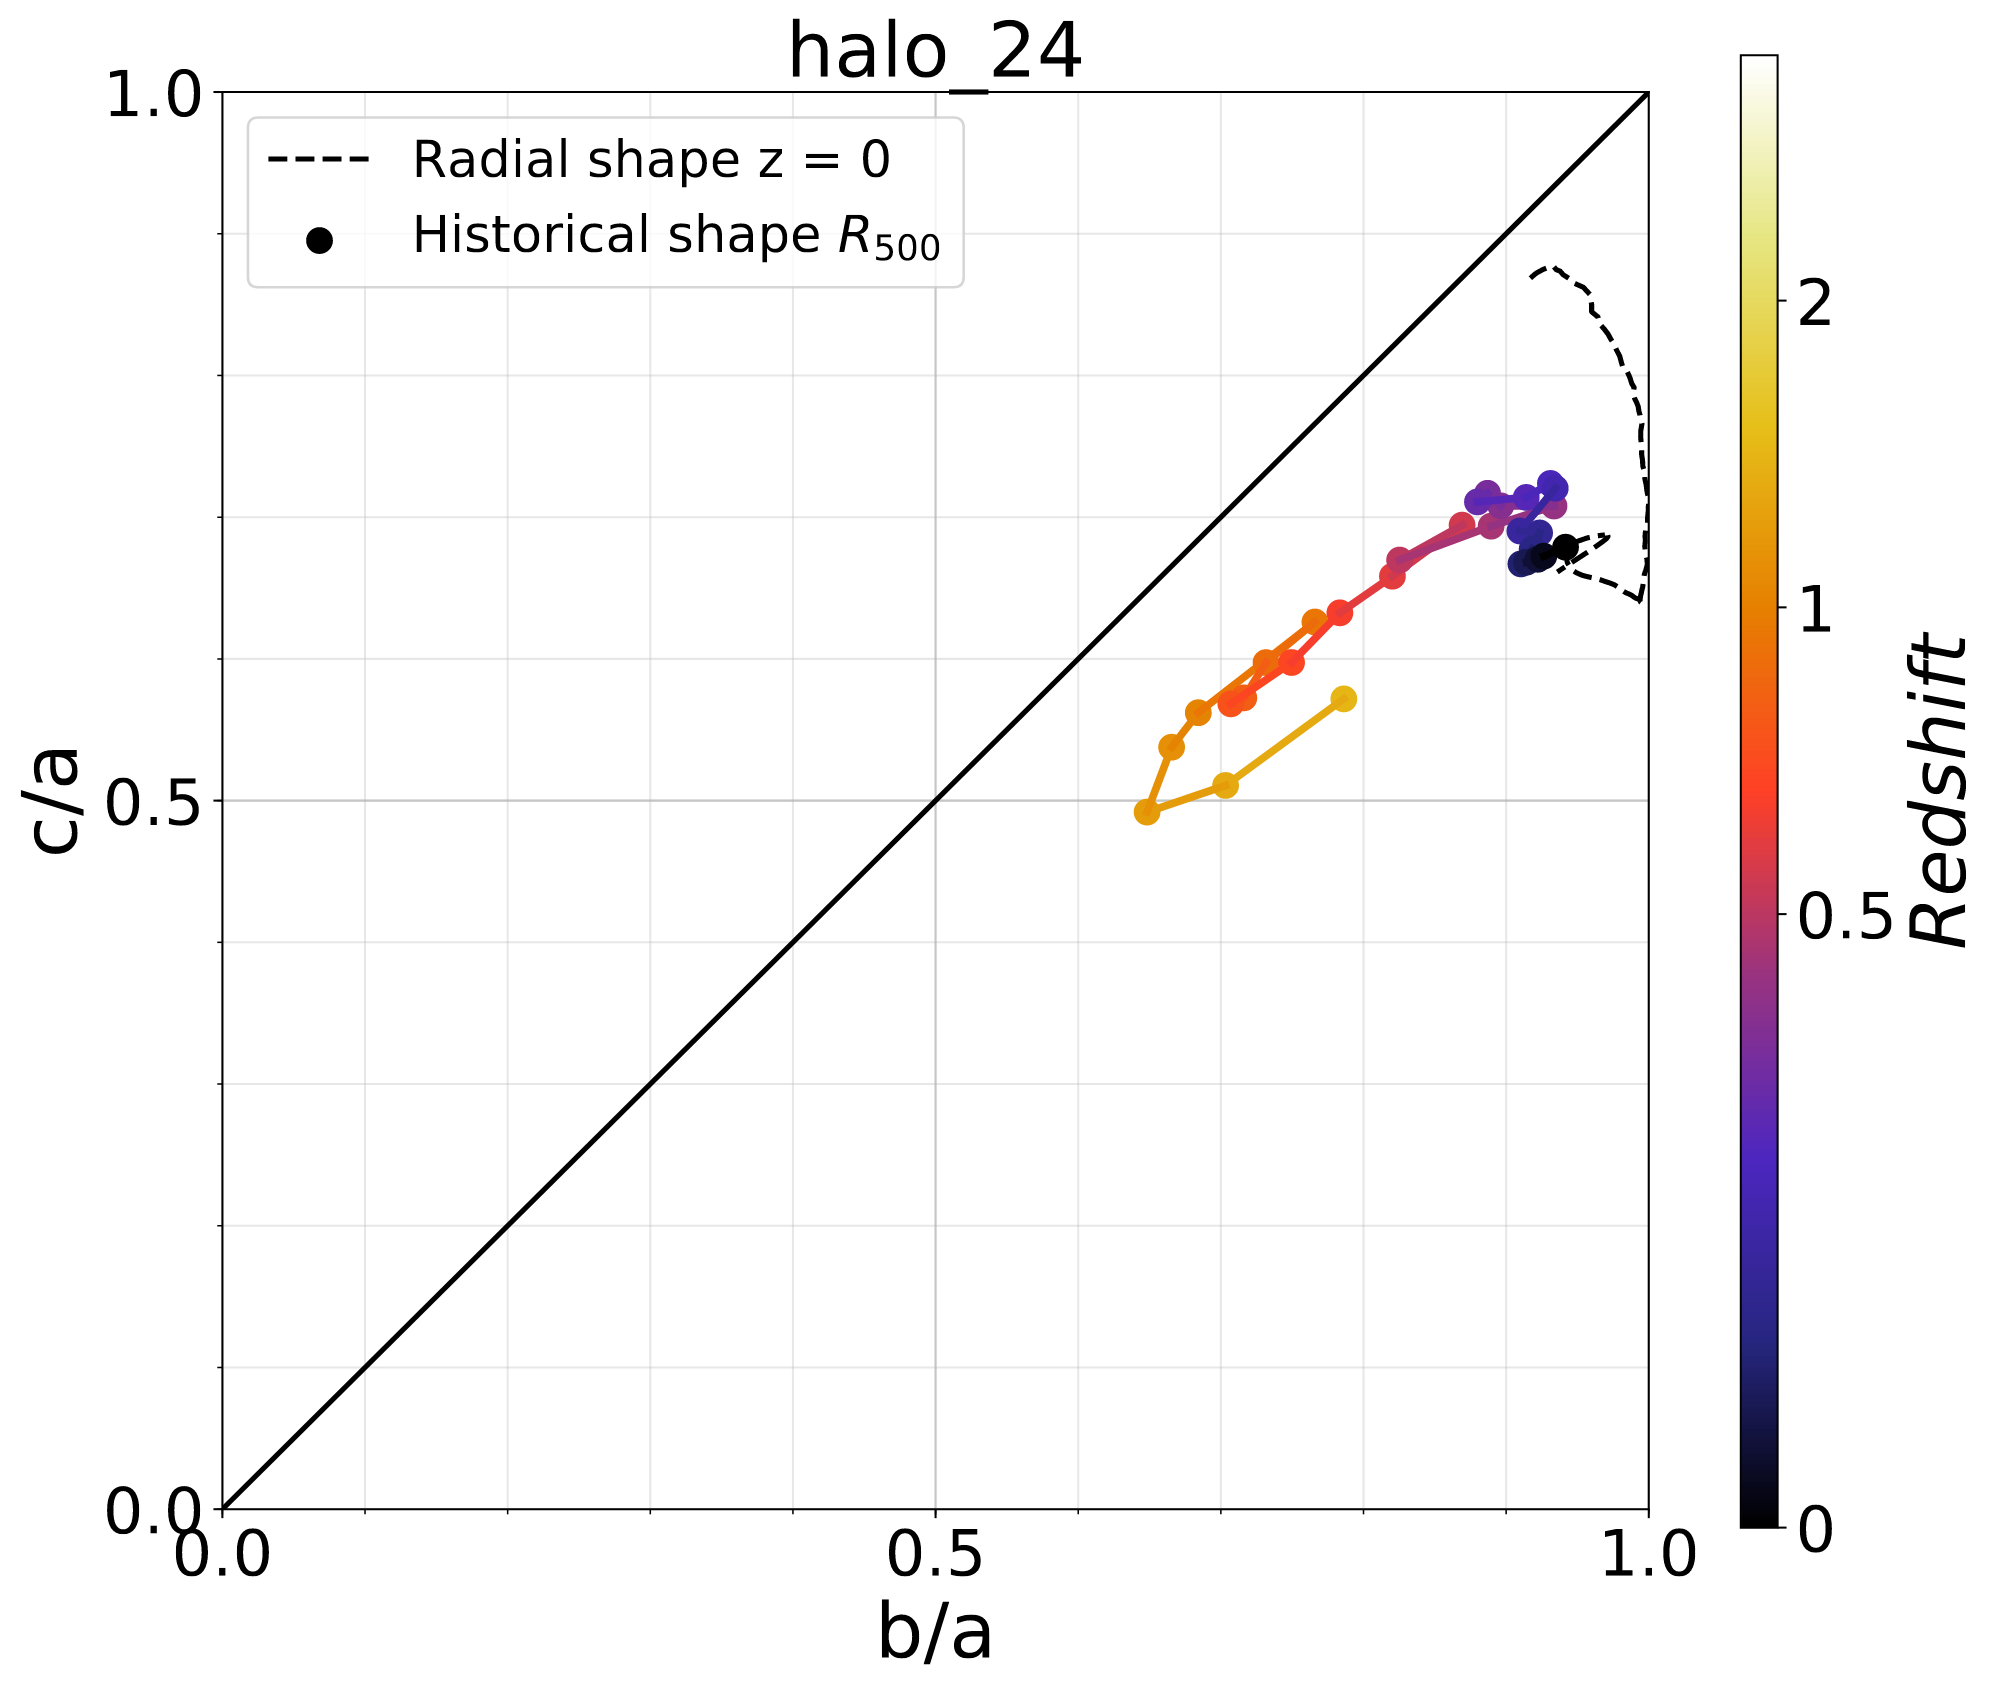
\includegraphics[width=\columnwidth]{./pics/Redshift/halo_24_level3_MHD_Z_Triax.png}
  \caption{Radial profile at $z=0$ (dashed line) and 
    the historical profile at the virial radius (colour line). 
    Results for DM simulations on the left, for MHD on the right.
    {\bf Aqui la idea es mostrar el mismo
      halo, no halos diferentes!}} 
  \label{fig:redshift_triaxial}
\end{figure*}

 
\begin{figure*}
  \subfloat[halo 16 DM]{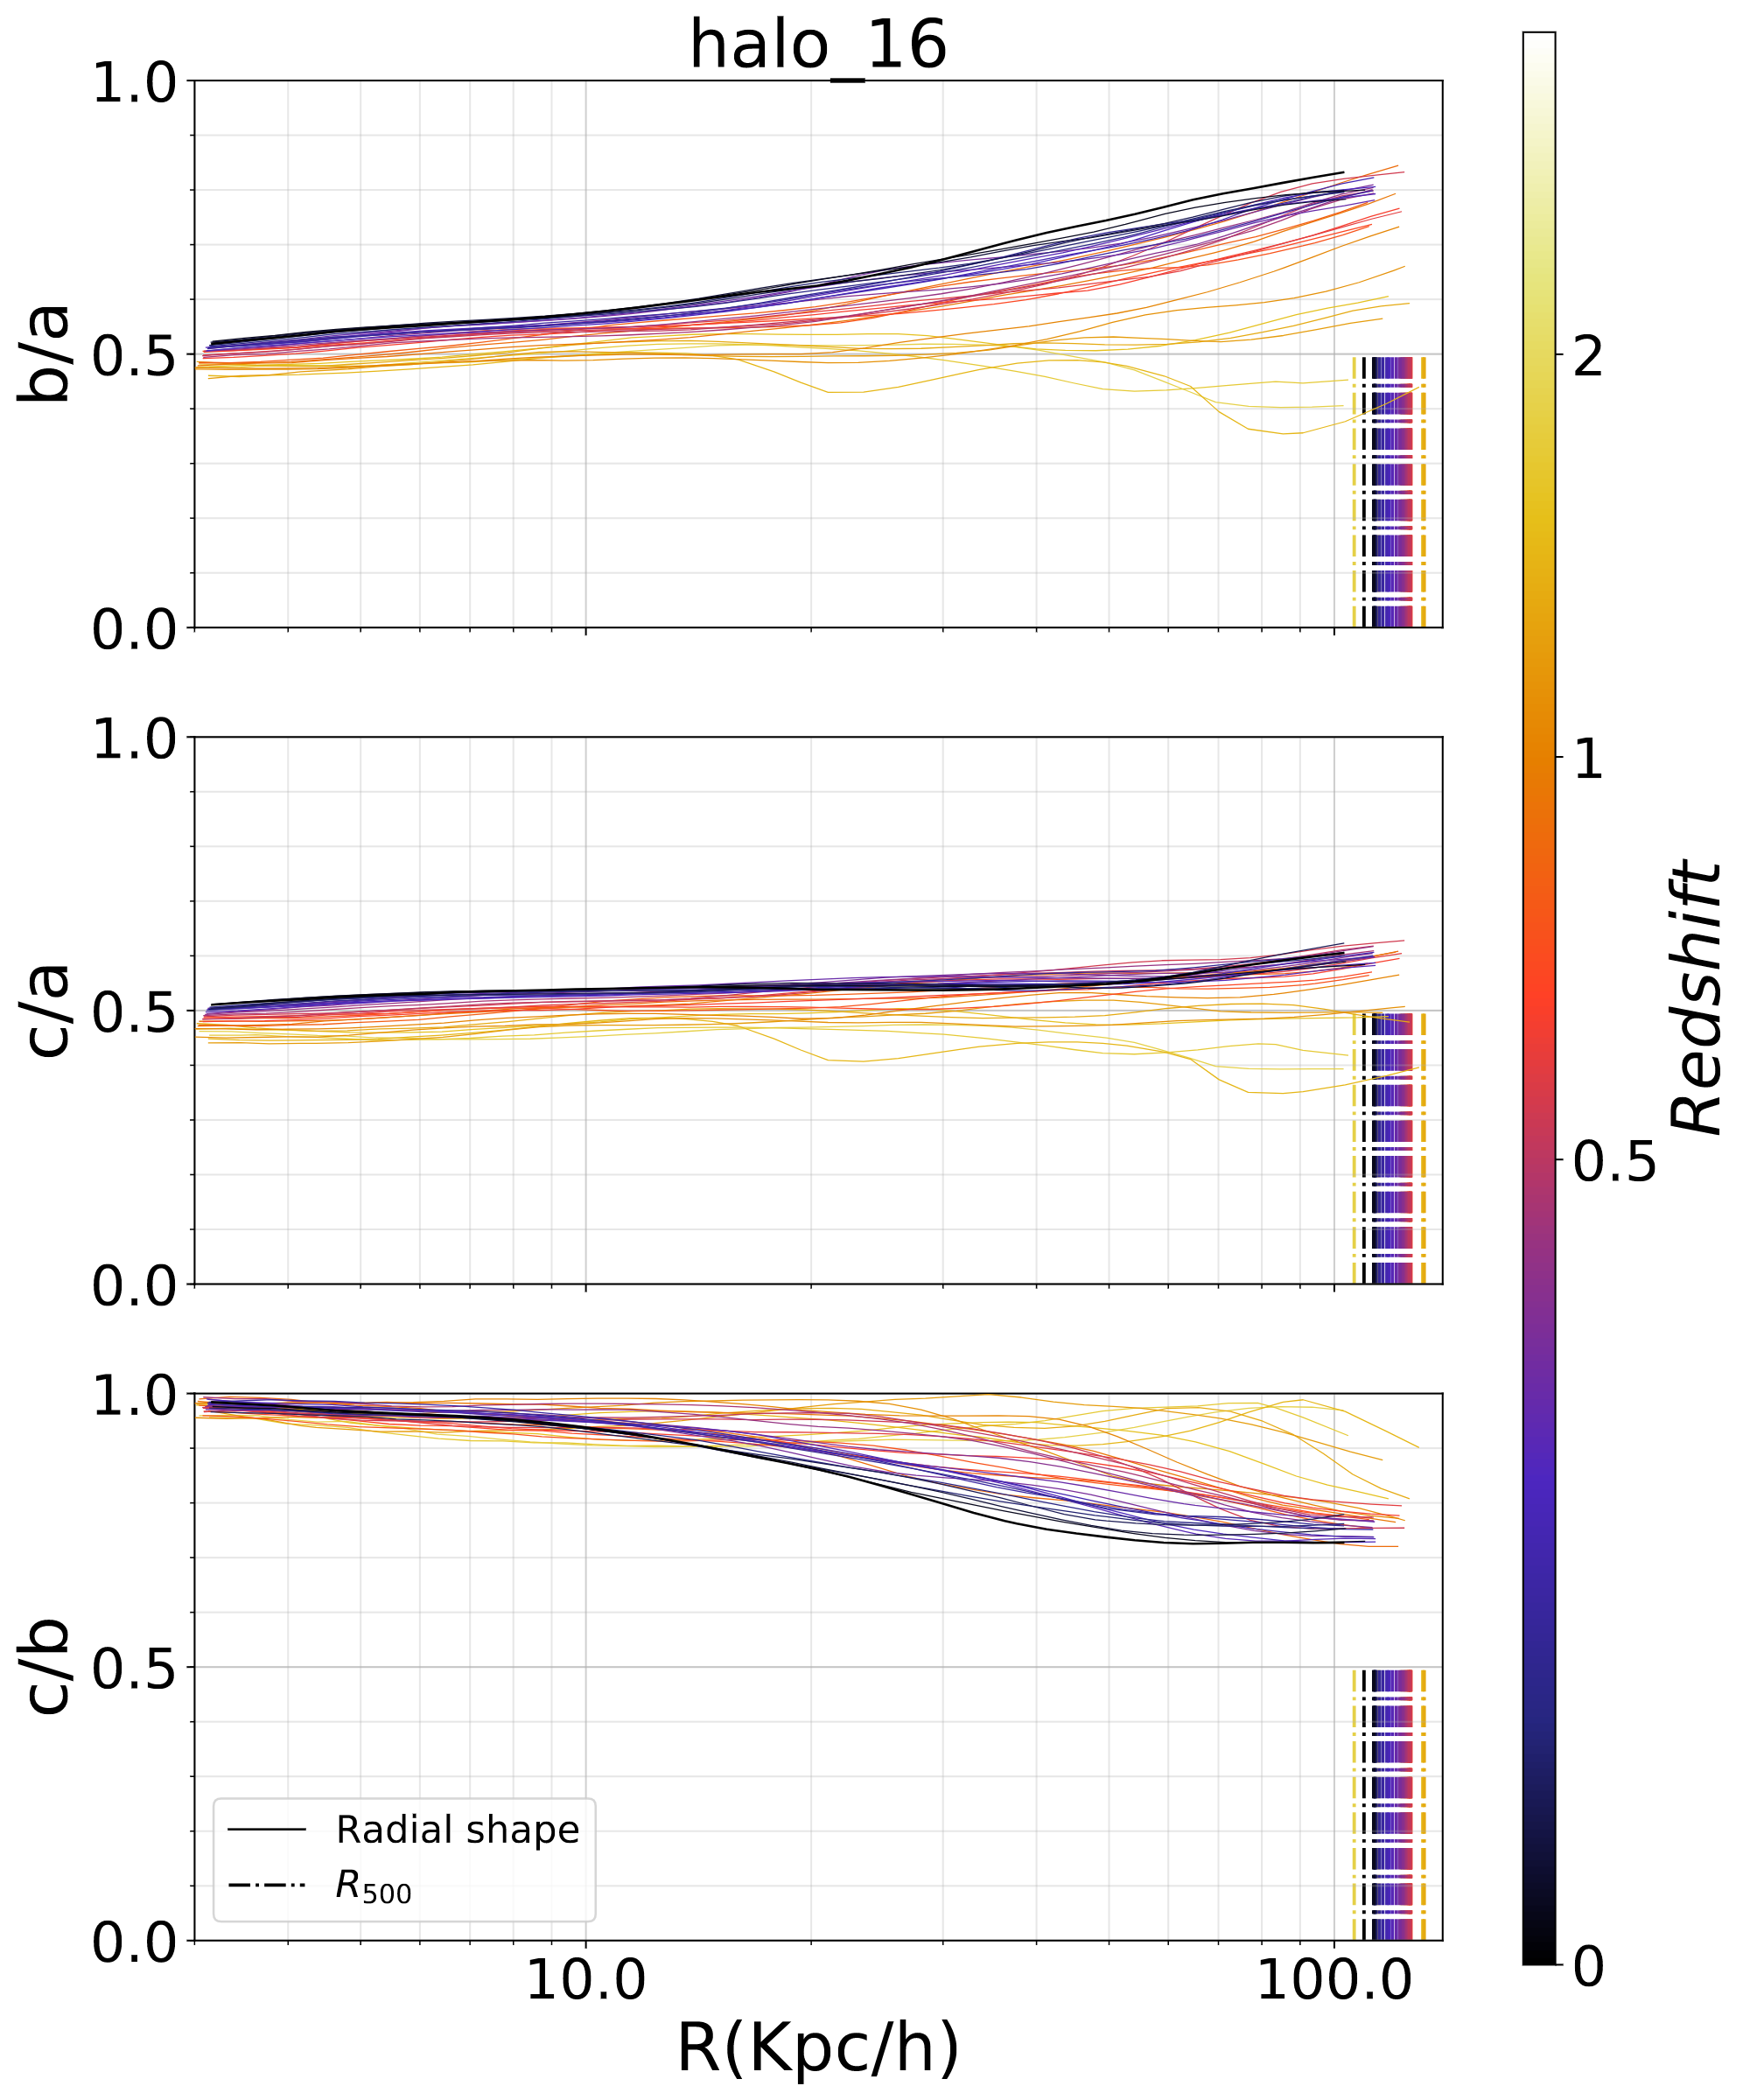
\includegraphics[width=\columnwidth]{./pics/Redshift/halo_16_level3_DM_Z.png}}
  \subfloat[halo 16 MHD]{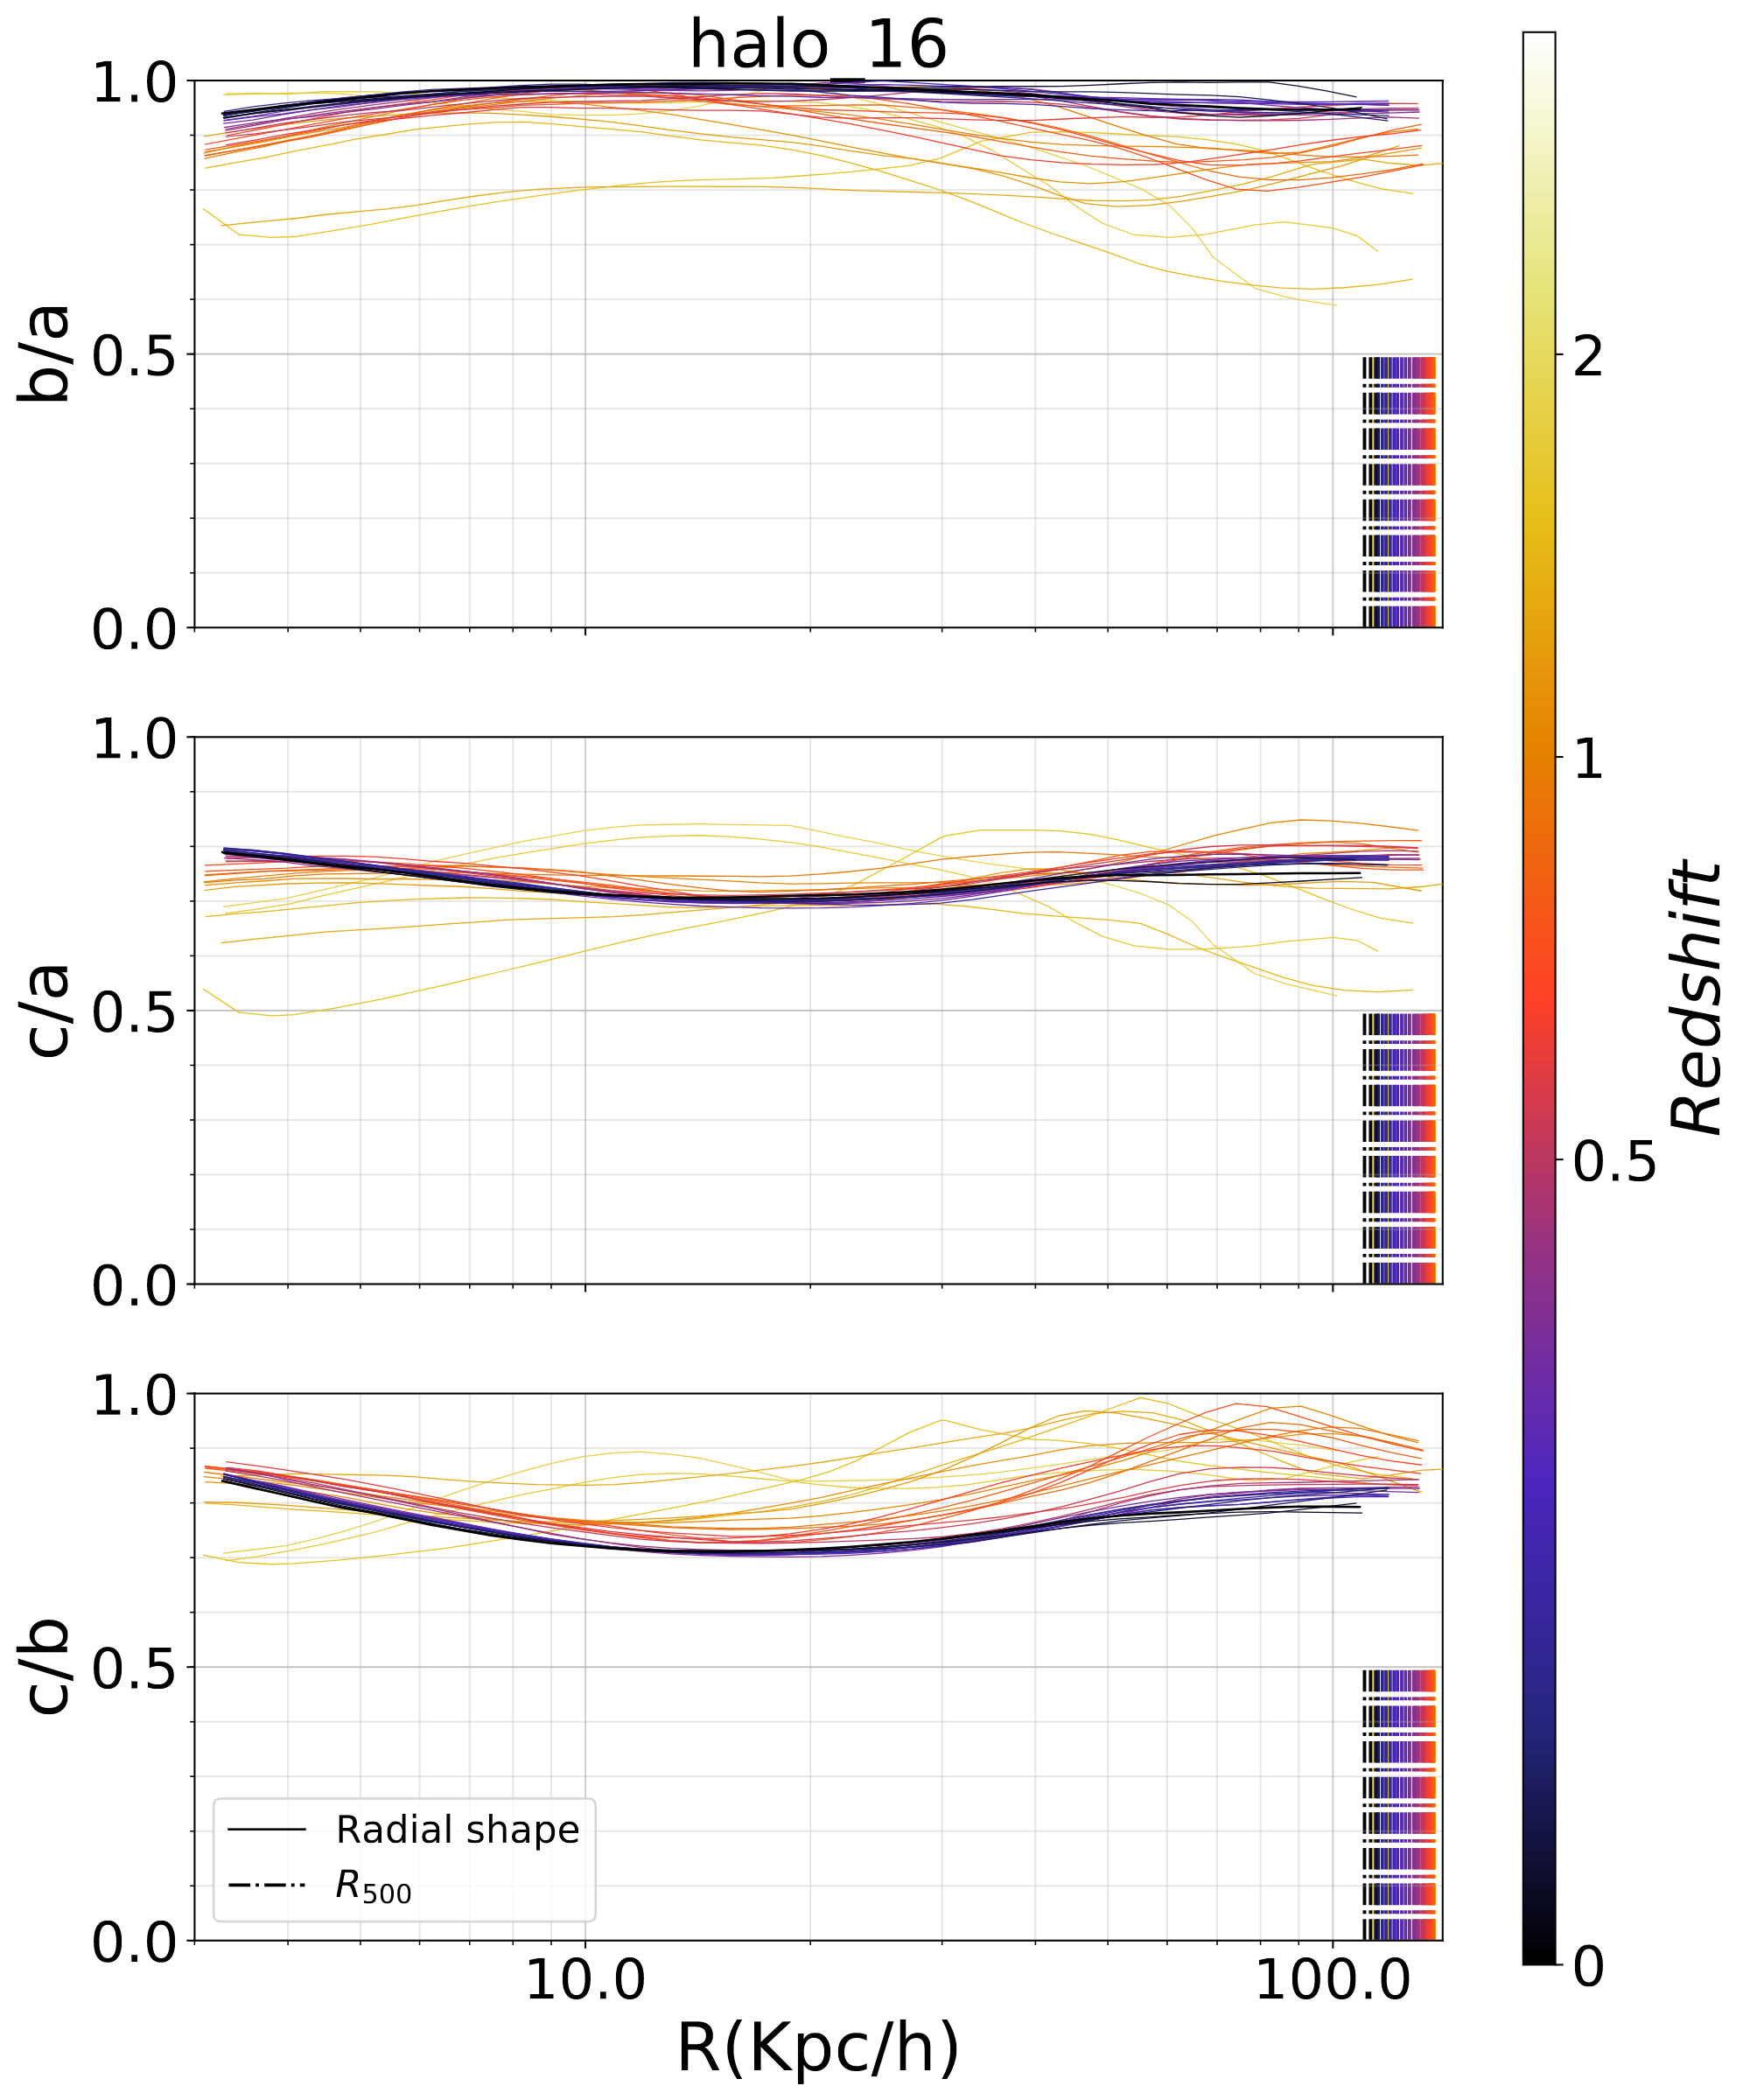
\includegraphics[width=\columnwidth]{./pics/Redshift/halo_16_level3_MHD_Z.png}}
  \caption{Radial profile (comoving) of axial ratios for halo 16 in
    terms of redshift (color). This halo maintains its shape until
    $z\approx 1$ obviating the systematic rounding effect in time from
    asymmetric potentials. Each plot-line represents the radial
    profile at a determined redshift. Conclussion: Mainly for b/a, it increases for:
    (1) for bigger radii (fixed redshift)(2) for lower redshift (fixed
    radius) It explains the correlation between radial profile and
    history, but does not require that curves match in the triaxial
    plane. {\bf En esta grafica el panel de abajo deberia ser la triaxialidad.}}
  \label{fig:RedshiftGood}
\end{figure*}

We know that DM-only have a steady and monotonous
trend towards larger sphericity with increasing radius. 
This radial trend is mimicked when the shape is measured at the virial
radius as a function of cosmic time.
The halo should become rounder with decreasing redshift, this is
expected by the continuous influence of the gravitational potential on
a collisionless fluid \citep{Vera-Ciro_et_al._2011}. 

We show in the left panel of Figure \ref{fig:redshift_triaxial} an
example with this effect in Halo 27 of the DM simulations:
the radial triaxiality at $z=0$ and the historical triaxiality at
$R_{\rm vir}$ are correlated. 
The right panel on the same Figure \ref{fig:redshift_triaxial}
illustrates how this correlation is absent in MHD simulations. 

This means that for DM-only halos one can approximate its shape at
higher redshift by simply sampling its 
current shape at a smaller radius. 
This correlation seems to be prompted by the continous inside-out
build-up of the dark matter halo; baryonic effects seem to jeopardize
the apparent smoother growth in DM-only simulations.

%Discuss if this correlation may be recovered if compared for example at Disk radius in stead of virial radius.\\


\subsection{DM halo - Stellar Disk Alignment}


A common assumption in observational models of the MW DM halo is that
its minor axis is perfectly aligned with the disk axis.
Although it is a reasonable assumption to guarantee the
stability of the galactic disk in simplified models of isolated
galaxies, this might not hold in an explicit cosmological context.

To examine the validity of this assumption  we sampled the shape at 5
different radii and plotted  directions in a cartesian coordinate
system where the $z$-axis always corresponds to the minor axis
measured at the virial radius.

{\bf En este caso hace falta la figura con la distribuci\'on integrada de cos theta}.
Figure \ref{fig:alignment} shows the cumulative distribution of
$\cos\theta$, where $\theta$ is the angle betwen the DM halo minor
axis and the stellar disk angular momentum.  
Each line shows the results at different radii.
We find that the majority of the disks are aligned with the minor axis
of their DM halo within $\approx 30^{\circ}$. 
Furthermore, if there is a good alignment measured at the virial
radius, this alignment is well conserved at smaller radii.

{\bf En este caso hace falta la figura de la evoluci\'on de cos theta
  como funci\'on del redshift}
However, there are some disks that show strong missalignments. 
To better understand the missalignments we plot the evolution of
$\cos\theta$ with time to find that the missalignment has been present
for the last XXX Gyr.
This trend is summarized in Figure \ref{fig:alignment_history}.

%\begin{figure*}
%  \centering
%  \subfloat[Perfectly aligned Axes]{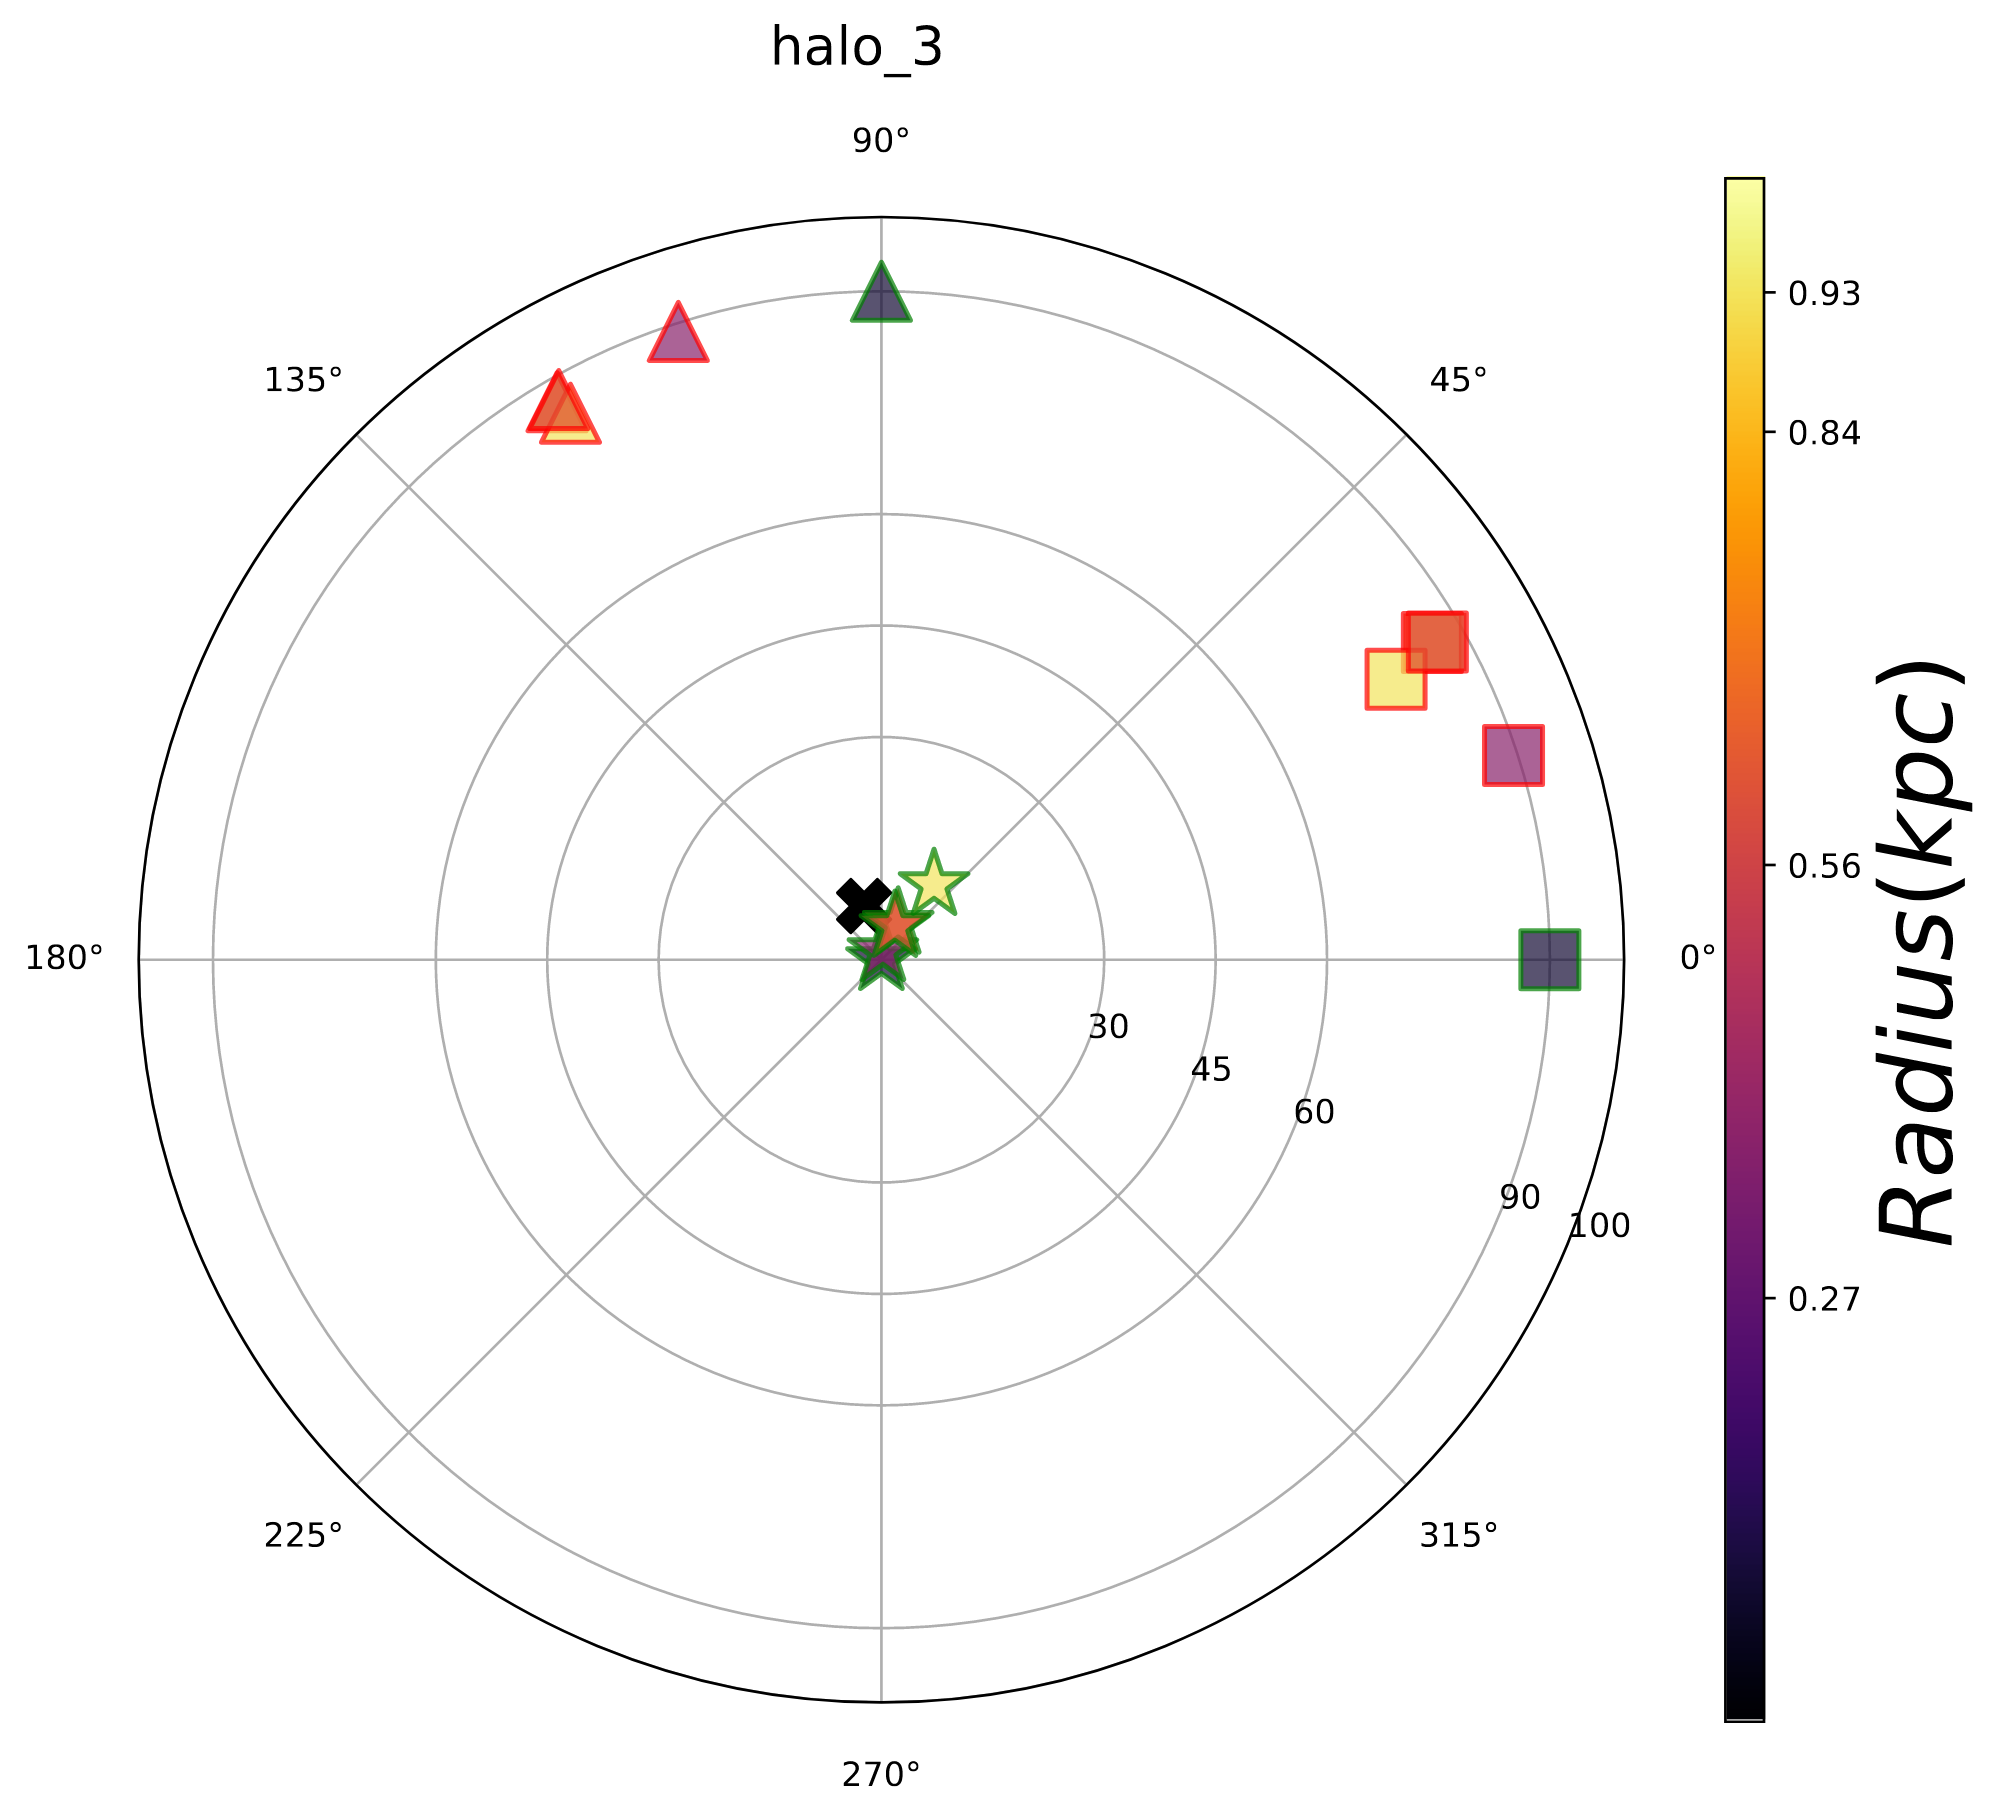
\includegraphics[width=0.6\columnwidth]{./pics/well_axes.png}}
%  \hfill
%  \subfloat[Somewhat aligned Axes]{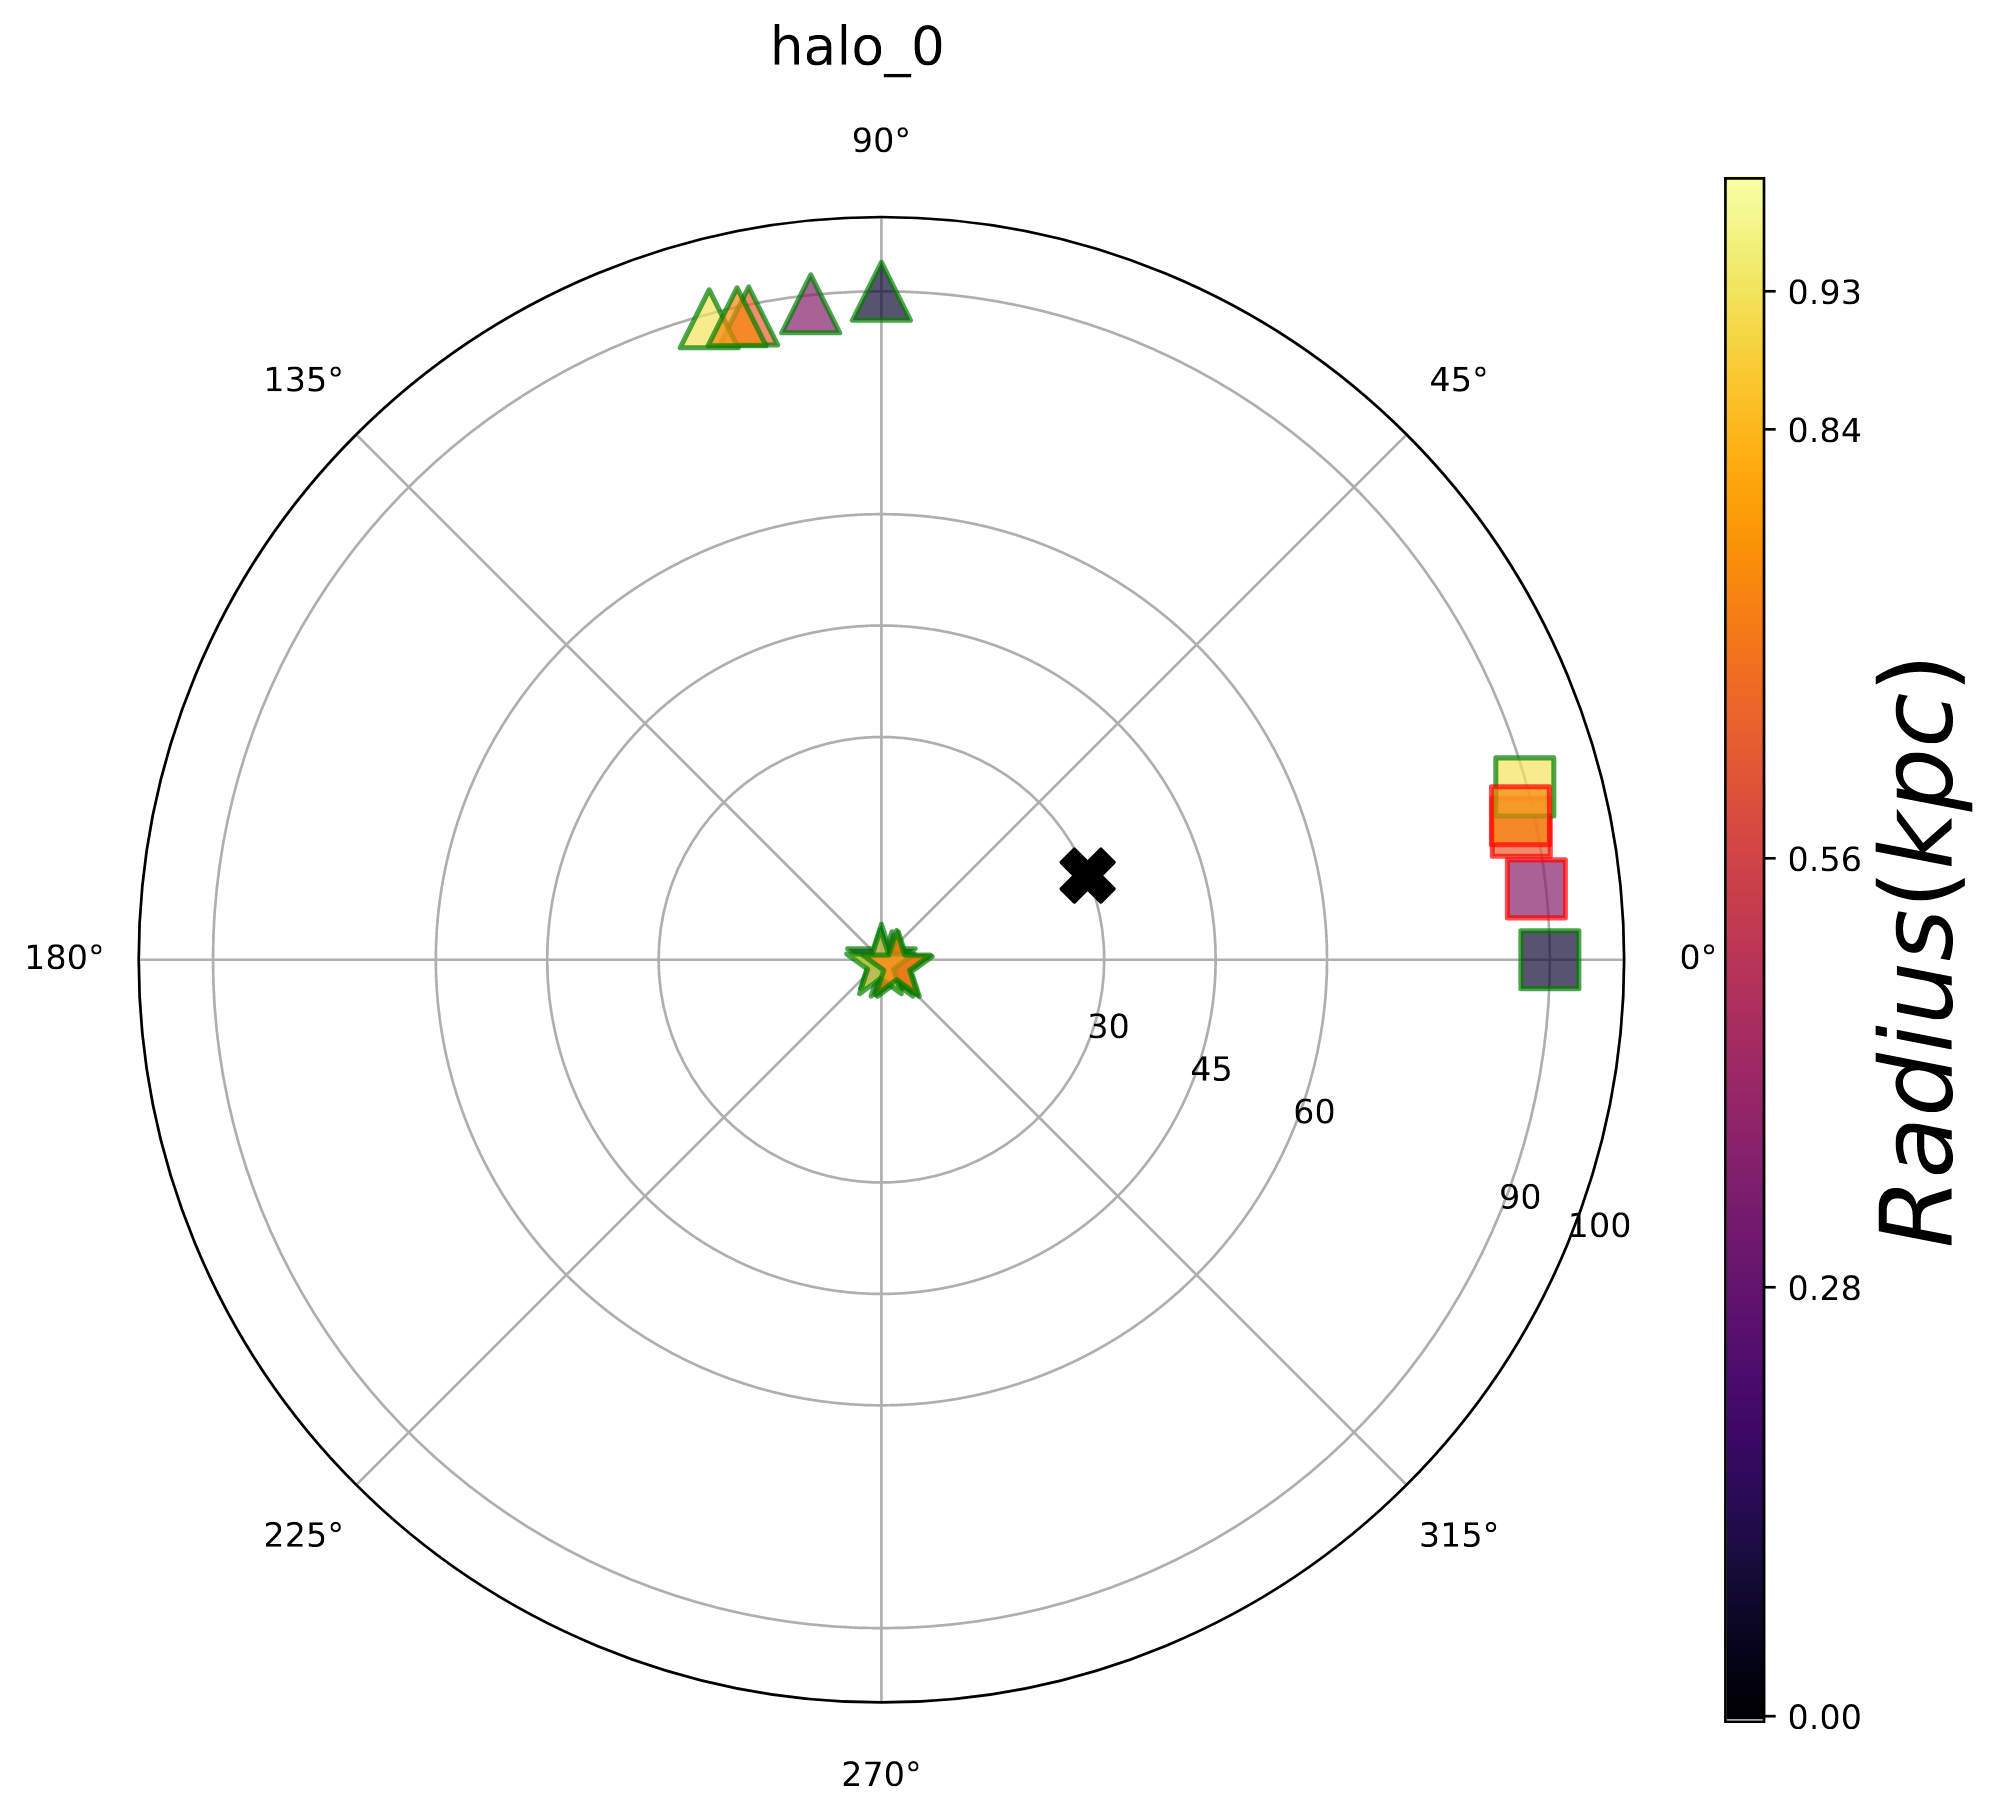
\includegraphics[width=0.6\columnwidth]{./pics/rotating_axes.png}}
%  \hfill
%  \subfloat[Chaotic Axes]{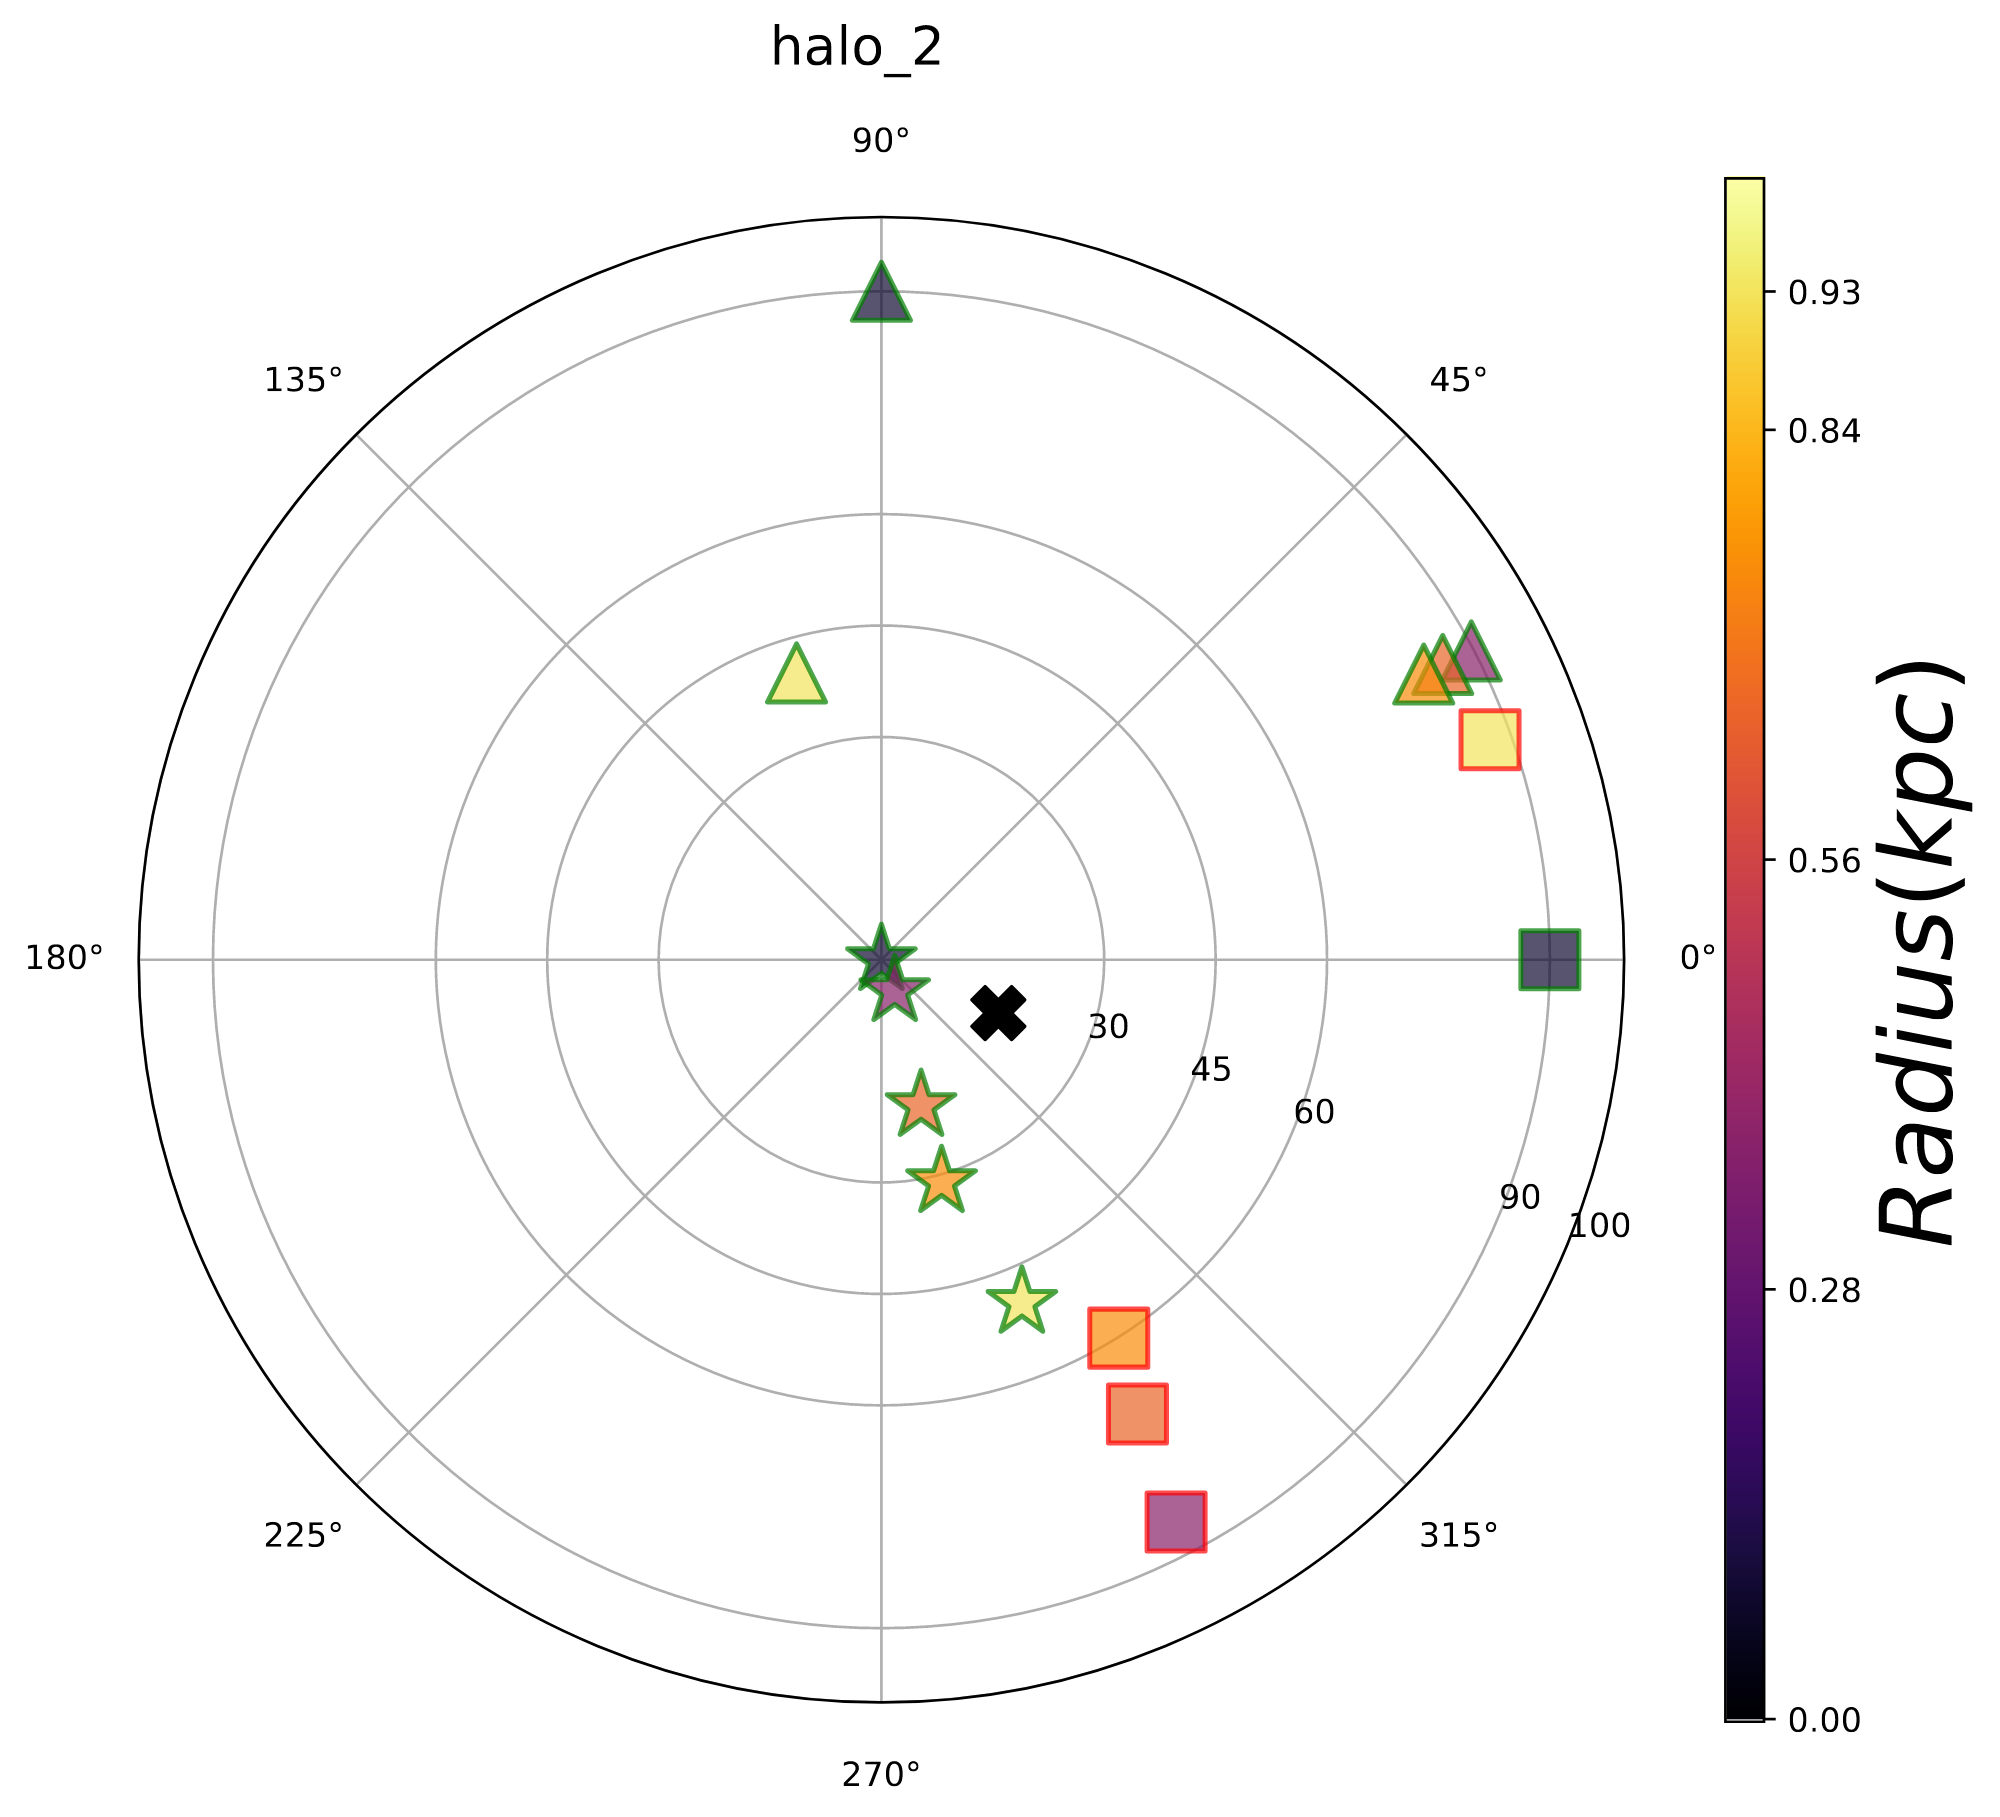
\includegraphics[width=0.6\columnwidth]{./pics/chaotic_axes.png}}
%  \hfill
%  \caption{Star: Minor Axis
%    Triangle: Medium Axis
%    Square: Major Axis
%    Color: Radii at which shape was sampled (show radii sampled)
%    Contour color: If orientation is above or below in this projection
%    Cross (black): Orientation of the stellar disk
%    Conclusion: Axes (minor) are not (generally) aligned with the
%    stellar disk nor are they usually aligned with each other from
%    different radii. We show some cases that may happen.} 
%  \label{fig:alignment}
%\end{figure*}

\textbf{Discussion about the distribution of alignments and their
  evolution in time: Precesion or temporary instabilities?} 

\section{Discussion}


\subsection{What drives the rounding effect?}

From our characterization of radial shapes it is clear that
MHD halos are rounder than DM halos every sampled radii. 
It is also noticeable that the rounding effect of baryons is stronger
at the disk regime, where the DM halo is almost perfectly oblate. 
Furthermore, MHD halos tend towards more oblate shapes (T < 0.5)
despite DM halos tendency towards more prolate shapes (T>0.5). 
This rounding effect can be explained by gravitational effect of the
flattened axisymmetric galactic disk. 
It also explanes the weakness of this affect around $\approx 100$kpc,
where the disk potential is weaker compared to the DM halo potential. 

{\bf Hace falta una grafica de la distribucion cumulativa de
  triaxialidad para (R\_vir y R\_vir/16 por separado), en cada panel se
  com para MHD vs DM.}
  
  \begin{figure*}
\centering
{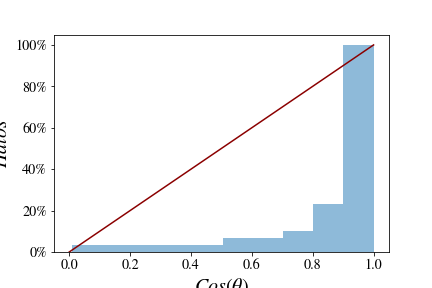
\includegraphics[width=0.6\textwidth]{./pics/Star_Disk_Alignment/Cummulative_Alignment_Histogram_Rvir.png}}
\caption{Cummulative distribution of alignment $cos\theta$ between the minor axis vector sampled as R virial and the star disk vector} \label{fig:alignment_out}
\end{figure*} 

  \begin{figure*}
\centering
{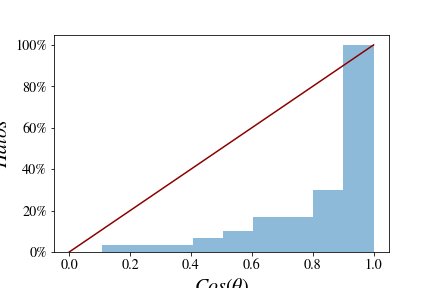
\includegraphics[width=0.6\textwidth]{./pics/Star_Disk_Alignment/Cummulative_Alignment_Histogram_Rvir_16.png}}
\caption{Cummulative distribution of alignment $cos\theta$ between the minor axis vector sampled as 1/16 of R virial and the star disk vector} \label{fig:alignment_in}
\end{figure*} 

Following that linea reasoning, one would also expect that the rounding
effect of baryons is related to some  galactic parameters such as its
component masses and radii. 
We look for these kind of correlations and to find that the strongest
can be found for the stellar density.
However, the correlation is relatively low ({\bf cuanto vale el
  coeficiente de correlation}) most likely due to the different
formation histories.
In other words, the effect of the baryonic disk on the shape of the DM halo
does not fully explain the deviation from oblateness of MHD halos at
$r<10$kpc. 

Figure  \ref{fig:Star_Density_effect} shows the
{\bf que es es lo que muestra esta grafica? falta las unidades de la
  densidad. y el eje vertical que es? es un cambio absoluto? fraccional?}

{\bf Finalmente cuales son las cantidades disponibles en el disco?
  cuales son las que muestran una mayor correlacion? Haria falta un
  plot con todas las correlaciones y la mencion de alguna prueba de
  machine learning del fit lineal para ver cuales son los parametros
  mas importantes.}

\textbf{Actually we have not examined the relation of c/a in MHD halos
  with some measure of c/a from the disk, that is something like
  Zdisk/Rdisk. This actually would make more sense from a physical
  point of view: effect of the potential. } 


\textit{ Talk about source of triaxiality at the inner parts of the
  halos (bar?). This source of triaxiality at the inner parts explains
  why the axial ratios are $\approx 0.95$ and not exactly $1$. We
  should also discuss that the decrease in the axial ratios for bigger
  radii may actually be bigger/steeper but it is dimmed by the
  contribution of inner parts.} 


\begin{figure}
  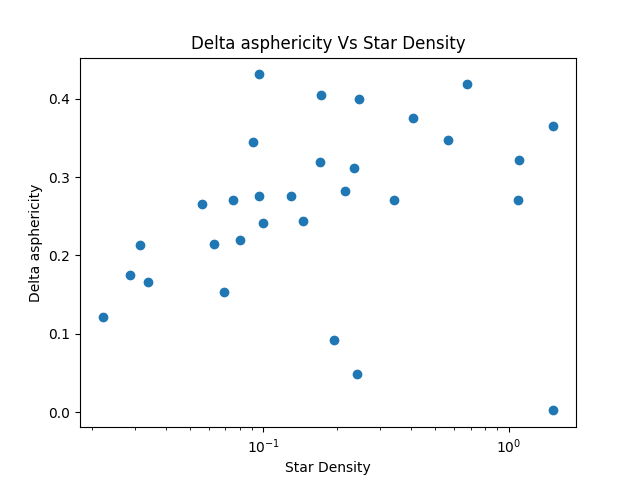
\includegraphics[width=\columnwidth]{./pics/Delta asphericity Vs Star Density.png}
  \caption{Difference in asphericities between MHD and DM shapes Vs
    Star Density of the simulation. Unsure about this graphic. Take
    delta asphericity as the strength of the rounding effect of
    baryons.}  
  \label{fig:Star_Density_effect}
\end{figure}



\subsection{Comparison against observational constraints}



\begin{table*}
\begin{tabular}{|l|cc|c|c|p{7cm}|}\hline
Reference&$q_{\rho}$&$s_{\rho}$&$R$&$\theta$&
Methodology\\ 
\hline \hline \citet{Olling_and_Merrifield_2000}& $1.00$
& $0.80$ &  $\simeq 8$kpc & $0^{\circ}$&Stellar dynamics and HI
density. \\

\multirow{2}{*}{\citet{Banerjee_and_Chanda_2011}}&${1}$&${1}$&$9$kpc&$0^{\circ}$&Method:
HI
gas. \\ &${0.5}$&${0.5}$&$24$kpc&$0^{\circ}$&Monotonical
change between radial regimes.\\

\citet{Loebman_et_al._2012}&${1.00}$&${0.47}$&$\sim
20$kpc &$0^{\circ}$&Method: SDSS statistics\\

\cite{Johnston_et_al._2005}&${1}$&$0.83-0.92$&$\lesssim
60$kpc&$0^{\circ}$&Method: Sagittarius stream\\

\citet{Bovy_et_el._2016}&${0.95}$&${0.95}$&$\lesssim
20$kpc&$90^{\circ}$ & Stellar streams\\

\citet{Deg_and_Widrow_2013}&$0.72$&$0.28$&
$20$kpc-$60$kpc$ $&$90^{\circ}$&
Mid-axis orientation. Sagittarius stream\\\hline\hline

\citet{Abadi_et_al._2010} &${0.98}$&${0.85}$& & & Simulations. Almost
  independent of radius. No feedback: boundary case\\\hline

\end{tabular}
\caption{{\bf Cuales son las incertidumbres? Con respecto a que eje
    esta medido theta?}}
\end{table*}


\begin{table*}
\begin{tabular}{|l|cc|c|c|p{7cm}|}\hline
Reference&$q_{\phi}$&$s_{\phi}$&$R$&$\theta$&
Methodology\\ \hline \hline 

\citet{Bowden_et_al._2016}& 0.5-0.66 &0.5-0.66& 5kpc - 10 kpc& $90^{\circ}$&
Weak constraint on prolate halo. SDSS stars dynamics.\\

\multirow{2}{*}{\citet{Vera-Ciro_and_Helmi_2013}}&${1.00}$&${0.90}$&$\lesssim
10$kpc&$0^{\circ}$ & Sagittarius stream \& LMC \\
&${0.90}$&${0.80}$&$\gtrsim 10$kpc&$90^{\circ}$&
Mid-axis orientation on the outside. \\

\citet{Law_and_Majewski_2009}&${0.83}$&${0.67}$&
$\lesssim 60$kpc&$90^{\circ}$&Mid-axis orientation. Sagittarius
stream\\

\citet{Law_and_Majewski_2010}&${0.99}$&${0.72}$&
$20$kpc-$60$kpc$$&$90^{\circ}$&Mid-axis orientation, Sagittarius
stream\\

\citet{Deg_and_Widrow_2013} & $0.82$&$0.40$&
$20$kpc $60$kpc$ $&$90^{\circ}$&
Mid-axis orientation. Sagittarius stream\\\hline \hline

\citet{Chua_et_al._2018}&${0.88\pm0.10}$&${0.70\pm0.11}$&$0.15R_{200}$&
& Illustris\\

\citet{Bryan_et_al._2013}&$0.84-0.86$&$0.66-0.70$&$R_{200}$& & 
For different cosmologies and feedback recipies. Calculated from a fit
at $M_\odot=10^12$\\\hline 

\end{tabular}
\caption{{\bf Cuales son las incertidumbres? Con respecto a que eje
    esta medido theta?}}
\end{table*}
%\end{multicols}



Half of the observational constraints are computed in terms of
isodensity contours, the other half in terms of isopotential contours.
To compare our results against the second kind we must either
translate the isodensity results or recompute in terms of isopotential
regions.
For this purpose, we run a simple iterative algorithm to find an
approximation of the shape of the isopotential contour. 

First, we calculate the mean and standard deviation of the potential over a
spherical shell of width equals to $10\%$ of the radius at which it is
sampled. 
Then, we calculate the inertia tensor of particles with potential
within $1\sigma$ around the mean potential and calculate its triaxial
characterization with the reduced inertia tensor. 
We repeat the
process of calculating the potential mean and standard deviation until
convergence is achieved with tolerance of $10^{-4}$. 

In Figure \ref{fig:density_potential} we compare the two approaches to
measure the axial rations and plot the analytic expectation for $q$, 
$(1-q_{\phi})\approx \frac{1}{3}(1-q_{\rho})$
\citep{Binney_and_Tremaine_2008}, taking the volume-enclosed axial
ratios  as an approximation for the isodensity contour ratios
$q_{\rho}$. 
This plot is computed at four different radii.

Although the analytic expression is meant to be used on the outer
regions of logarithmic axisymmetric halos, it works well as a first
approximation for nearly axisymmetric halos as those produced by our
simulations 
We find that the difference between the measured and the
approximated isopotential axial ratios is not bigger than $quantity
percent$ {\bf }. 


{\bf Aqui hace falta una grafica comparando explicitamente los
  valores para q y para s, esto para diferentes radios.
  Otro punto importante es que se tiene q, pero como se
  relaciona s?
  Ademas hay que calcularlos para los radius aproximados que se
  presentan en las tablas observacionales y en las de simulaciones.
  10-20kpc se acerca a 1/8Rvir, 20-25 1/4Rvir, 60kpc aproximadamente 1/2Rvir
}

\begin{figure*}
\centering
{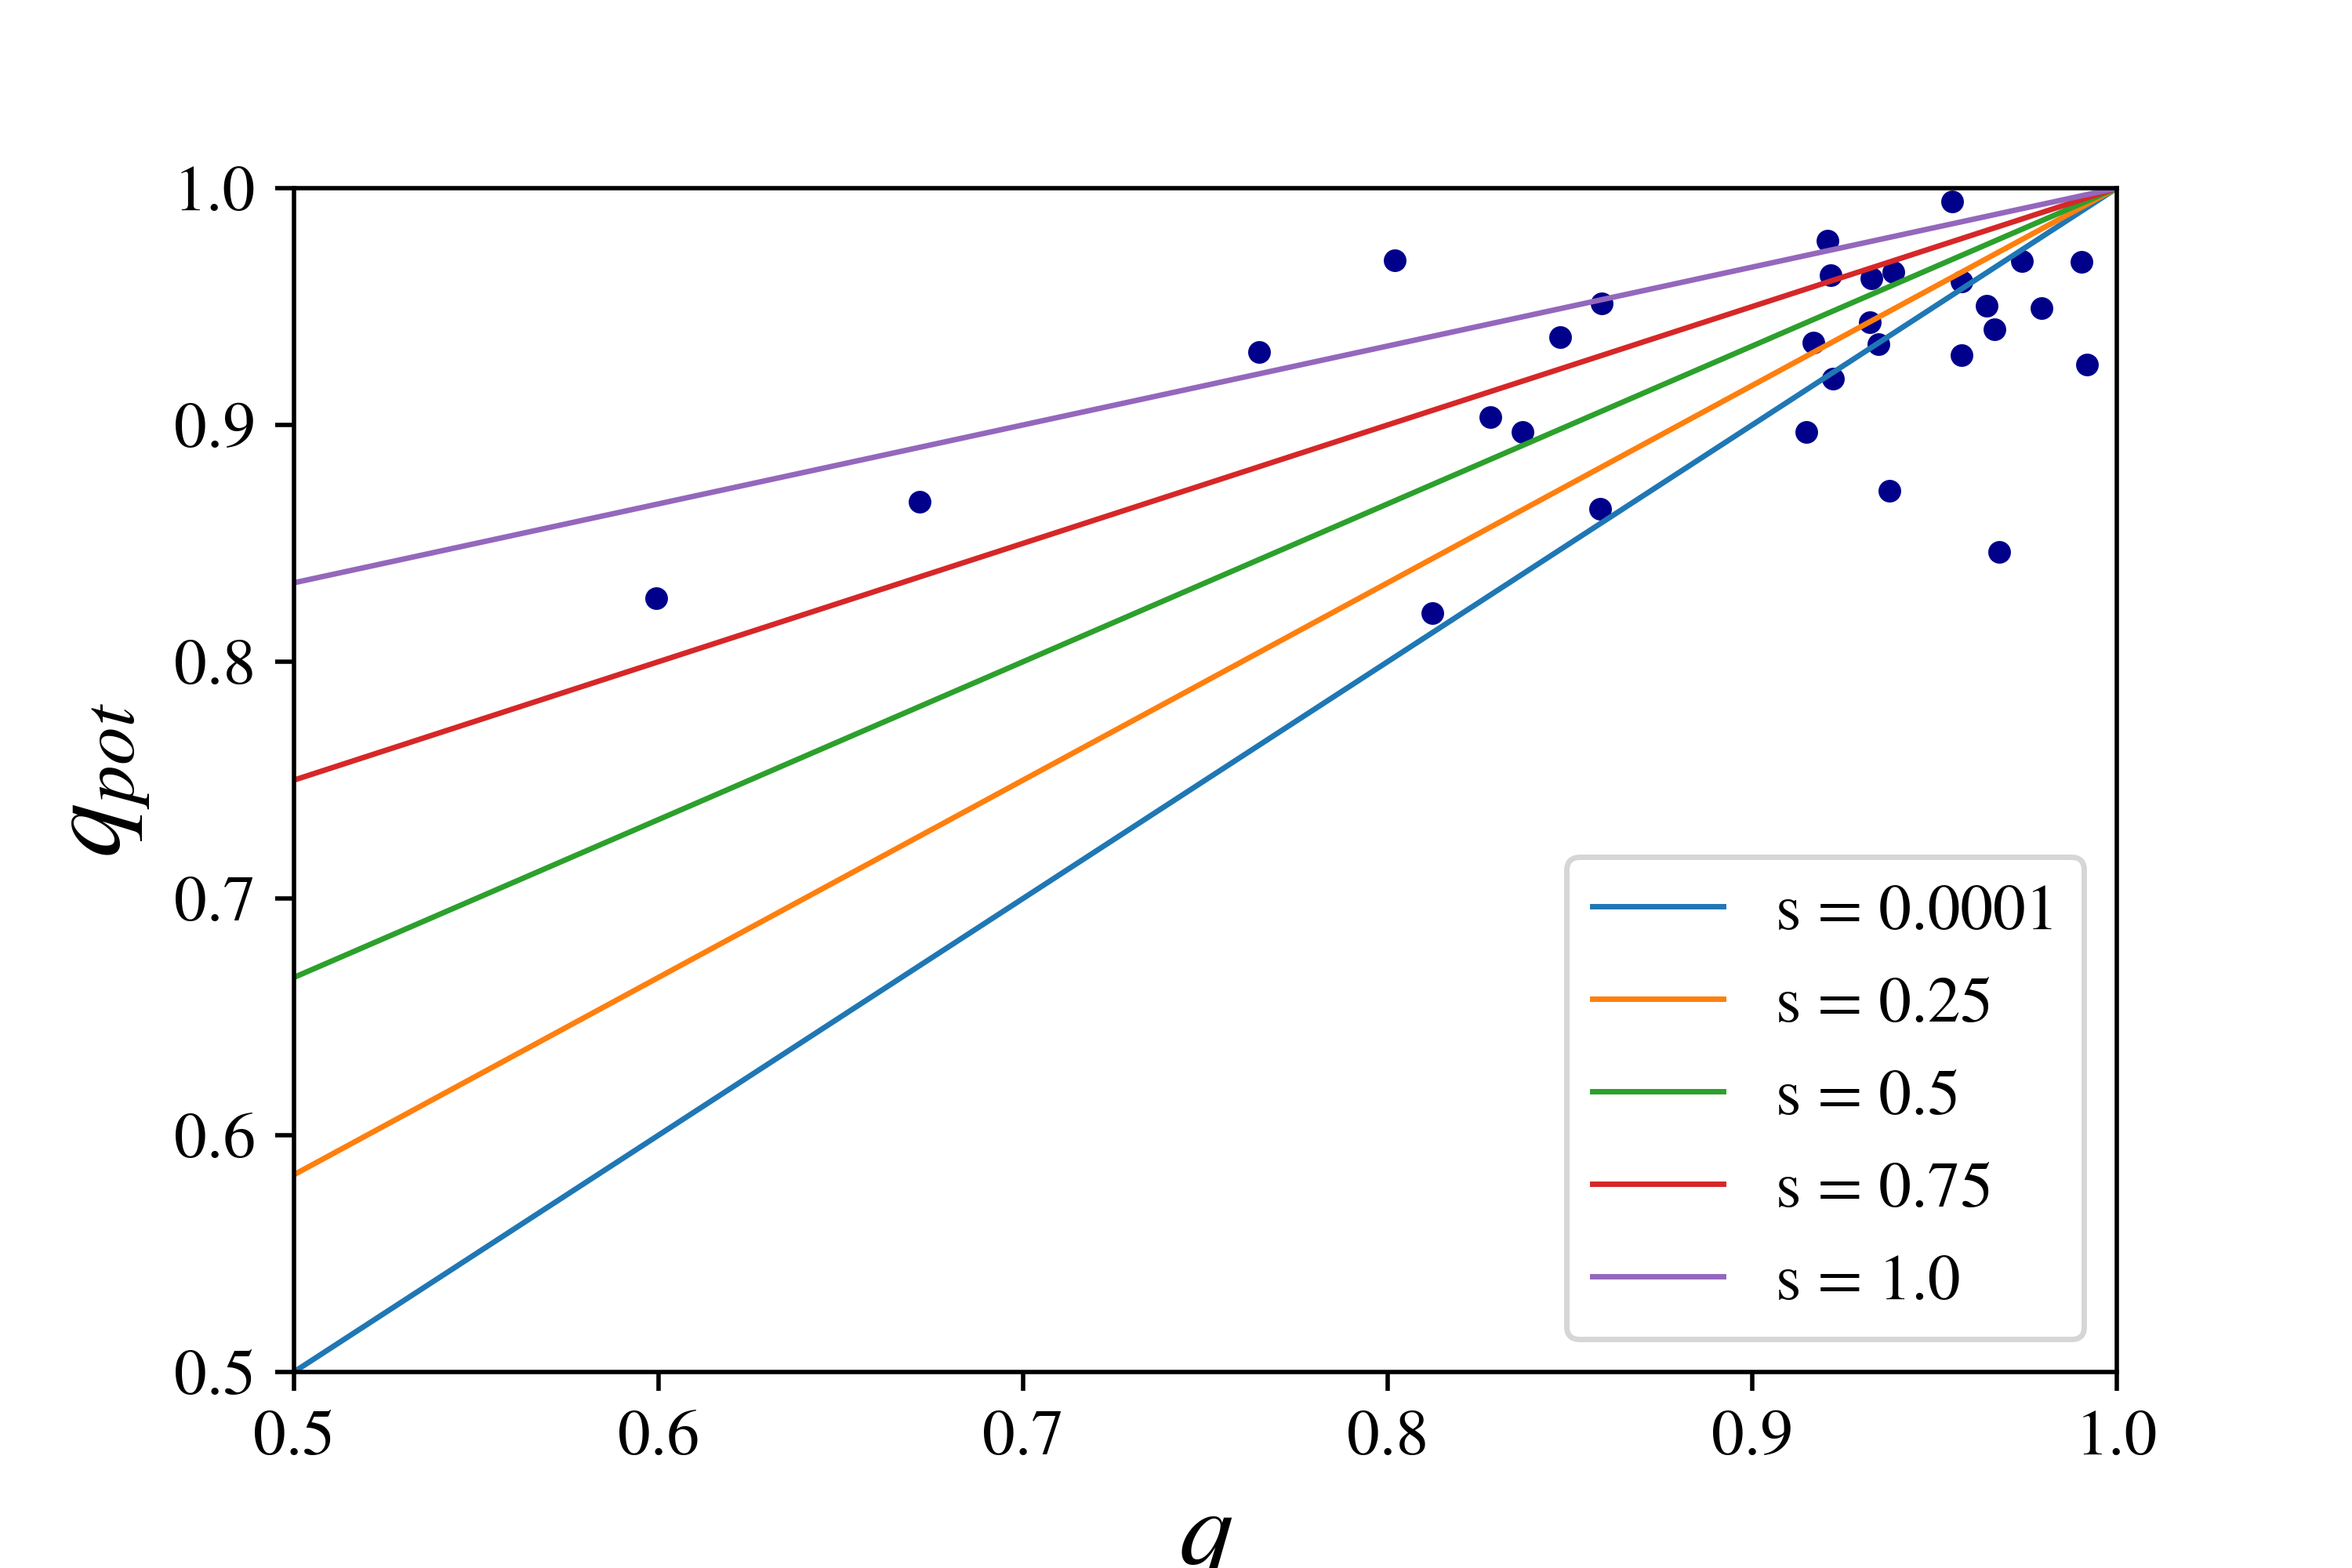
\includegraphics[width=0.6\textwidth]{./pics/Shape_Methods/q_pot_Vs_q_den.png}}
\caption{Comparison of q calculated with isopotential and with density enclosed volumes. Continuous lines represent the Binney and Tremaine approximations for different ratios s. Scatter points represent the calculated shapes with an isopotential approximation and with the Allgood method} \label{fig:shape_comp}
\end{figure*} 

\begin{figure*}
\centering
{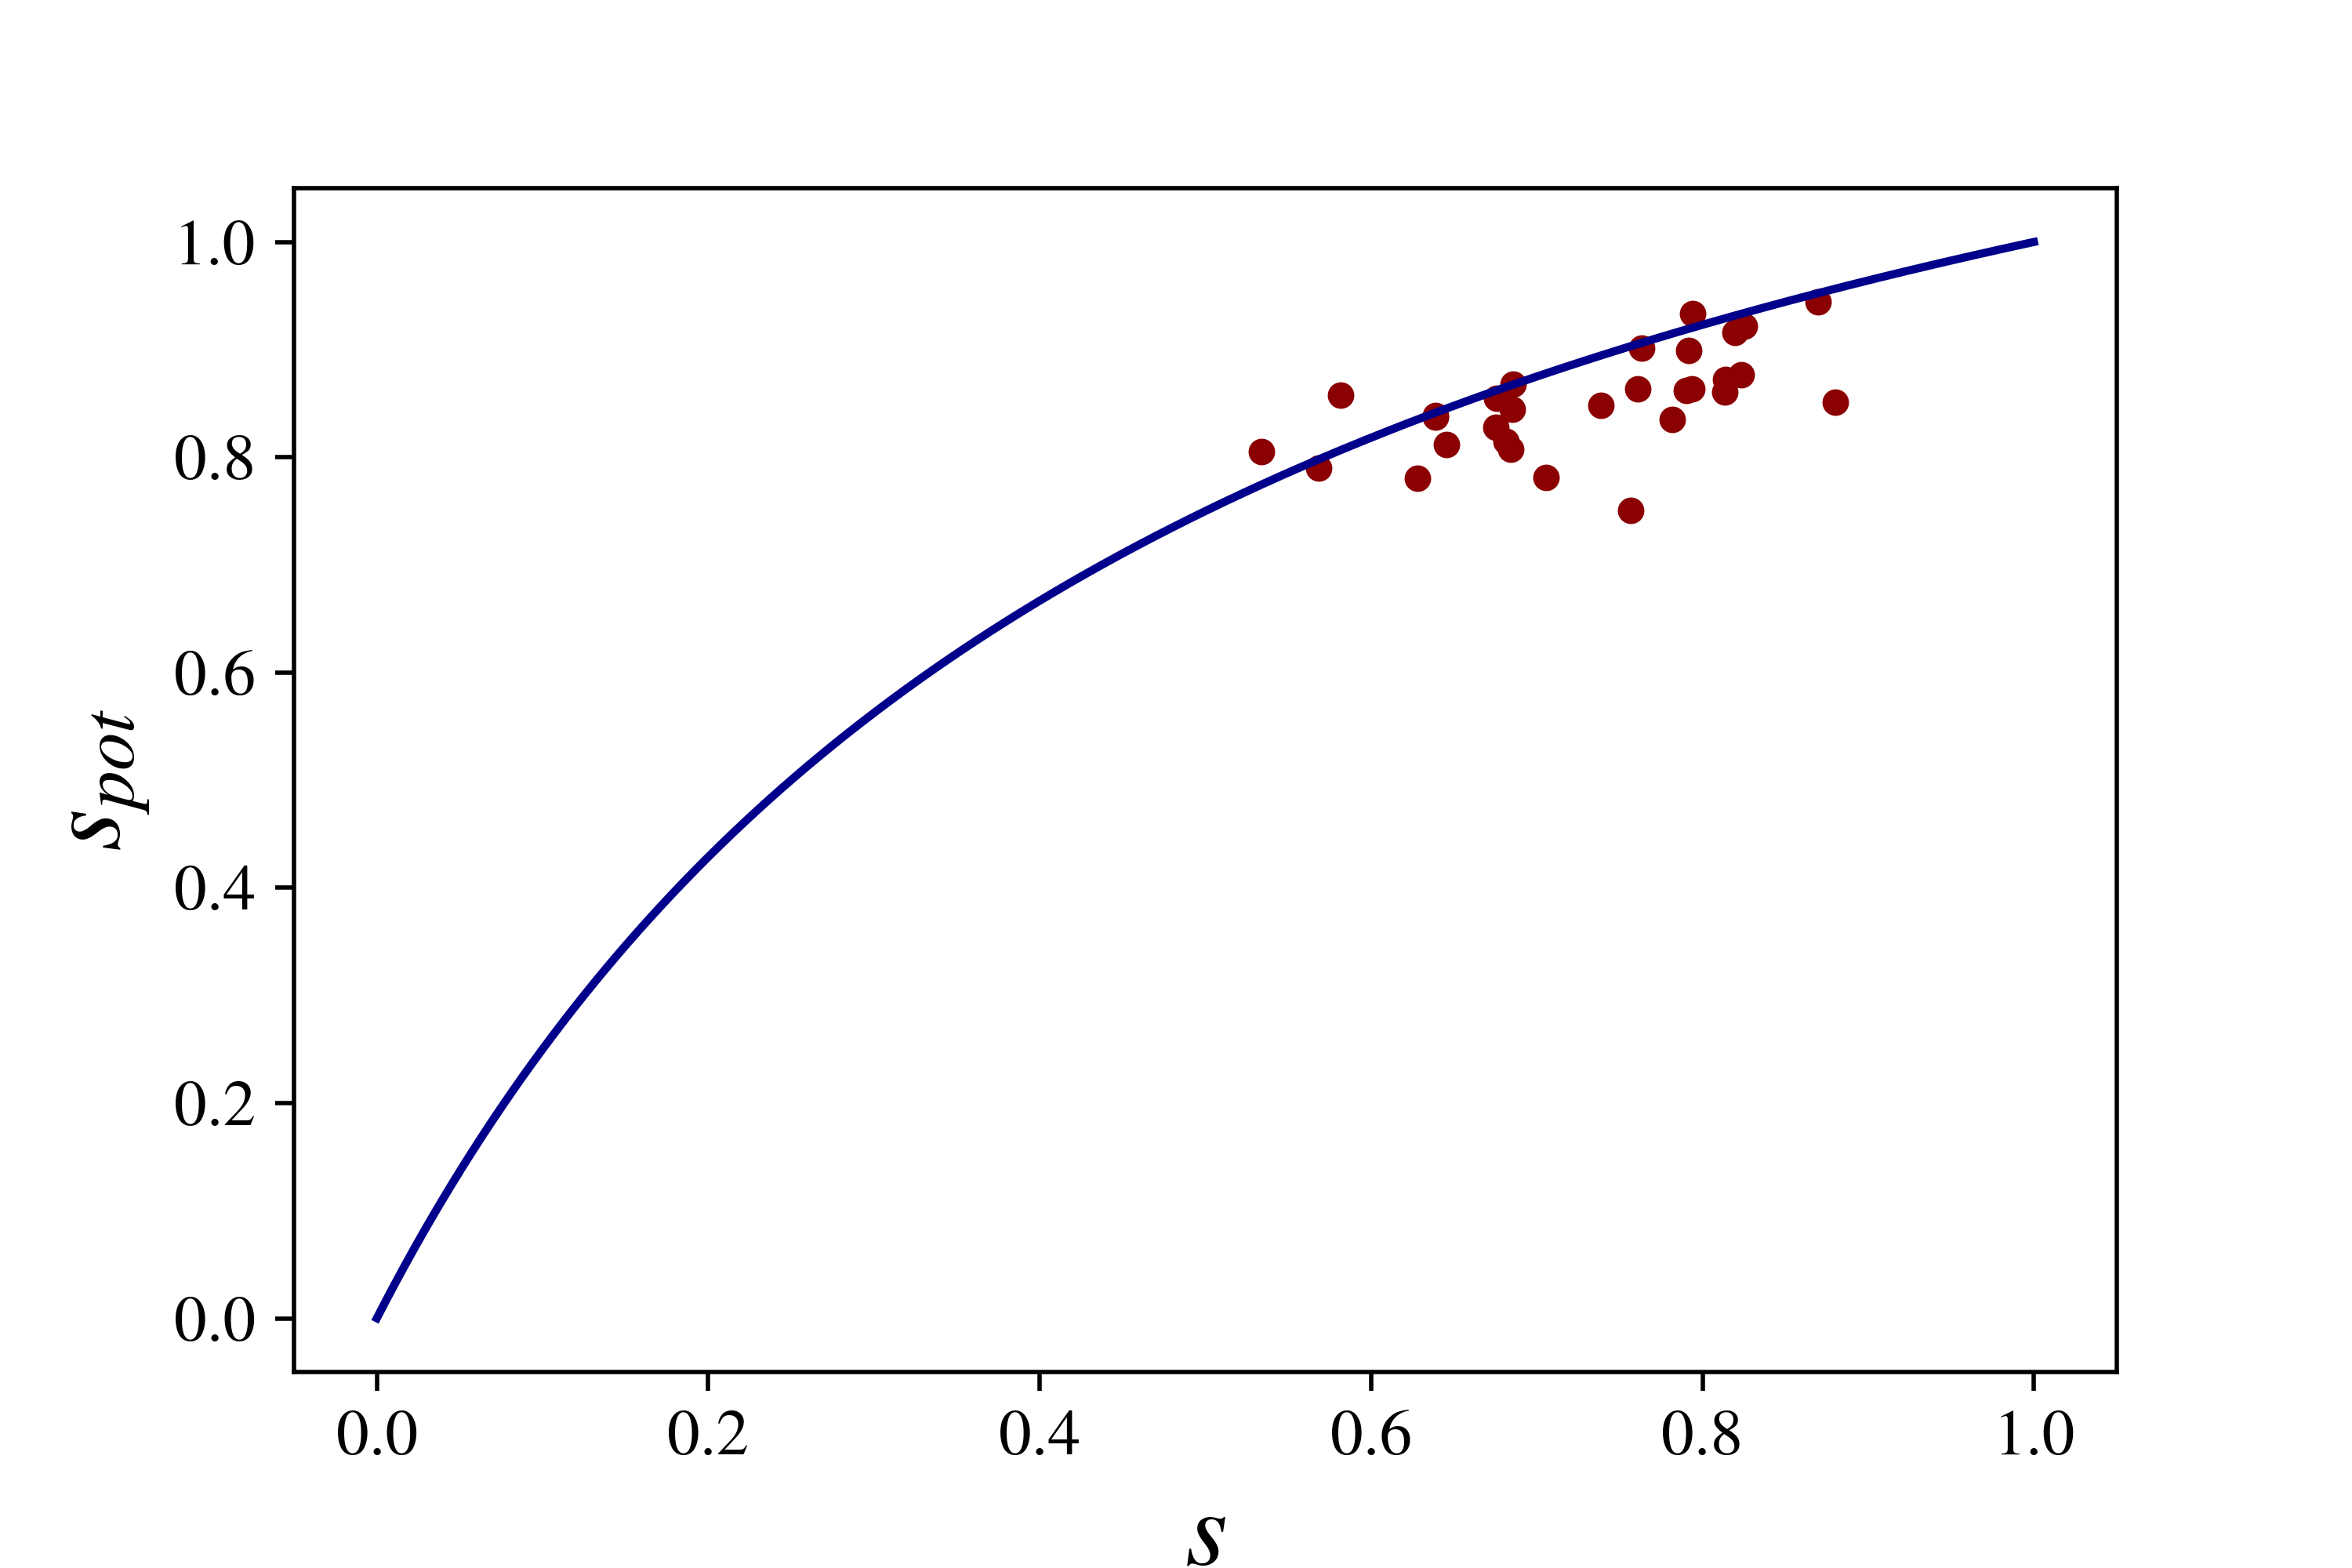
\includegraphics[width=0.6\textwidth]{./pics/Shape_Methods/s_pot_Vs_s_den.png}}
\caption{Comparison of s calculated with isopotential and with density enclosed volumes. Continuous lines represent the Binney \& Tremaine approximation. In the case of the ratio s, it does not depend on q.ds Scatter points represent the calculated shapes with an isopotential approximation and with the Allgood method} \label{fig:shape_comp}
\end{figure*} 



\begin{table}
\setlength{\tabcolsep}{3pt}
\begin{tabular}{l|cccc}
 & $R_{1/8}$& $R_{1/4}$& $R_{1/2}$& $R_1$ \\
\hline \hline
$\bar{q}$&$0.98^{+0.01}_{-0.02}$&$0.97^{+0.01}_{-0.04}$&$0.96^{+0.03}_{-0.06}$&$0.94^{+0.03}_{-0.07}$ \\[0.1cm]
$\bar{s}$&$0.89^{+0.04}_{-0.06}$&$0.88^{+0.04}_{-0.04}$&$0.87^{+0.05}_{-0.05}$&$0.85^{+0.05}_{-0.05}$ \\[0.1cm]
$\bar{T}$&$0.18^{+0.23}_{-0.10}$&$0.36^{+0.19}_{-0.21}$&$0.40^{+0.26}_{-0.20}$&$0.48^{+0.23}_{-0.21}$ \\[0.1cm]
\hline
\end{tabular}
\caption{Median values of isopotential axial ratios $q,s$ and triaxiality parameter $T$ for DM halos in MHD simulations at different radii (columns). }
\label{tabe:isopotential}
\end{table}


\section{Conclusions}


\section*{Acknowledgements}
This project has received funding from the European Union's Horizon
2020 Research and Innovation Programme under the Marie
Sk\l{}odowska-Curie grant agreement No 734374. 

 \bibliographystyle{mnras}
 \bibliography{references}
\end{document}
